\hypertarget{ch2}{%
\chapter{Physiographic controls and sensitivities of midwinter snowpack in Sierra Nevada, CA}\label{ch2}}

\hypertarget{ch2-abstract}{\section{Abstract}\label{ch2-abstract}}

% Significance and motivation
% Research goal and questions
% Methods
% Key findings
% Context sentence

Seasonal snowmelt from midlatitude mountain environments is the primary source of water for nearly a billion people globally. With recent climate change, midwinter melt events caused by snow droughts and dry spells are becoming more common. Yet, physiographic parameters (i.e., elevation, aspect, and slope) are first-order controls of fluxes of water and through the environment, complicating the impacts of these climatic variations. For a more comprehensive understanding of how snowpacks will react to warming temperatures across spatial scales, we must quantify the physiographical controls and climatological sensitivities of important hydrological snowpack metrics. To do this, we used the high-resolution spatiotemporally complete Sierra Nevada Snow Reanalysis (SNSR) dataset from 1985--2016. Using three distinct study basins, we analyzed four physiographic snowpack metrics and tested their sensitivities to meteorologic forcings. We quantified marked differences in snow accumulation and ablation between aspects, basins, and elevations. On average, south-facing slopes displayed four times more in midwinter melt than north-facing slopes. These results display. Our results also showed that aspect plays a key role in climate sensitivity, especially at higher elevations. This displays that physiographic variables play an important role in the snowpack's response to future warming. This study produced the first quantified estimates of climatic-scale physiographic-based snow metric variability for the climate-sensitive snowpacks of the Sierra Nevada. It also highlights the importance of spatially-distributed, fine-resolution snowpack data for understanding highly variable snowpack processes in mountain regions.

%==============================================================================
%==============================================================================
%==============================================================================
\hypertarget{ch2-intro}{\section{Introduction}\label{ch2-intro}}
\hypertarget{ch2-intro-1}{\subsection{Significance and Motivation}\label{ch2-intro-1}}


Seasonal snowmelt from midlatitude mountain environments is the main source of water for nearly a billion people across the globe \citep{sturmWaterLifeSnow2017}.
Climate warming is affecting the stationarity of various hydroclimatic processes \citep{millyStationarityDeadWhither2008}. In the western United States (WUS), this means warmer winter temperatures \citep{gergelEffectsClimateChange2017}, more cold season precipitation falling as rain \citep{knowlesTrendsSnowfallRainfall2006}, which in turn impact snow accumulation and ablation processes \citep{kapnickCausesRecentChanges2012}. These snowpack variations influence streamflow timing \citep{stewartChangesSnowmeltRunoff2004} and affect the magnitude of streamflow overall \citep{barnhartSnowmeltRateDictates2016}. Hydroclimatic changes pose significant implications for water resources management in an uncertain future \citep{livnehDroughtLessPredictable2020}.

Common snow metrics like April 1st snow water equivalent (SWE) and maximum SWE (MSWE) are used to estimate spring flows \citep{paganoEvaluationOfficialWestern2004}. With recent climate change, midwinter melt events caused by snow droughts \citep{harpoldDefiningSnowDrought2017} and dry spells \citep{hatchettMidwinterDrySpells2023} are becoming more common. This melt impacts MSWE, ablation season processes, and streamflow generation. Both \cite{harpoldHumidityDeterminesSnowpack2018} and \cite{musselmanWinterMeltTrends2021} showed the importance of midwinter melt, but their studies relied on point-based station data. Specifically, \cite{musselmanWinterMeltTrends2021} states that to better understand the impact of anthropogenic warming on snow, it is important to continue investigating the relationship between climatology, physiography, and snowpack. This allows for more insights into how snowpacks will react to warming temperatures across spatial scales, as this still remains unclear \citep{molotchEstimatingDistributionSnow2008}. Therefore, we must quantify the physiographical controls and climatological sensitivities of hydrologically important snowpack metrics.

% -----------------------------------------------------------
\hypertarget{ch2-intro-2}{\subsection{Background}\label{ch2-intro-2}}
\hypertarget{ch2-intro-3}{\subsubsection{Key physiographic parameters}\label{ch2-intro-3}}


In mountain regions, physiographic parameters (i.e., elevation, aspect, slope) are first-order controls of fluxes of water, energy, and nutrients through the environment \citep{pelletierWhichWayYou2018a}. Aspect, or slope orientation, serves as a primary control on hydrologic, ecologic, and geomorphic processes, as it moderates the intensity of incoming solar radiation (herein, insolation) \citep{broxtonRoleAspectQuantify2009}. Net shortwave radiation is the primary driver of snowmelt in the ablation season \citep{marksClimateEnergyExchange1992a}. Insolation variability is amplified in midlatitude mountain environments, where lower sun angles create large differences between north and south-facing slopes. 

% -----------------------------------------------------------
\hypertarget{ch2-intro-4}{\subsubsection{Limitations of previous work}\label{ch2-intro-4}}


Spatial and temporal scales of observations need to be relevant to the physical process of interest. For instance, \cite{bloschlScalingIssuesSnow1999} showed that the relevant spatial scale for snow hydrology in mountain regions $\sim$100~m, with this resolution showing the ability to resolve critical spatial characteristics. Past studies have leveraged long-term point-based in situ data \citep{clowChangesTimingSnowmelt2010,harpoldChangesSnowpackAccumulation2012a,kapnickCausesRecentChanges2012,musselmanWinterMeltTrends2021} and kilometer-scale models to evaluate various climatic-scale monotonic snowpack metric trends 
\citep{moteDECLININGMOUNTAINSNOWPACK2005, moteDramaticDeclinesSnowpack2018, zengSnowpackChange19822018, haleDriversSpatiotemporalPatterns2023}. However, snow pillows cover less than 1~\% of the land area and are limited to mainly mid-elevation flat forest cuts \citep{guan20102011Snow2013}. Additionally, macroscale hydrologic models (e.g., Variable Infiltration Capacity (VIC) \citep{liangSimpleHydrologicallyBased1994}) or snow reanalyses (e.g. UA daily 4~km SWE product \citep{broxtonLinkingSnowfallSnow2016}, SNOw Data Assimilation System (SNODAS) \citep{barrettNationalOperationalHydrologic2003}) have resolutions on the scale of kilometers. This makes neither of these data well-suited for understanding snowpack patterns in complex topography. \cite{trujilloSnowpackRegimesWestern2014} used SNOTEL data from the WUS to characterize distinct geographic snowpack regimes, yet physiographic variables were not considered due to data limitations.

%%% studies that do use aspect! (elder???) 
Few past studies have considered physiography in their characterization of mountain snowpack. In a detailed field study of a small alpine watershed, \cite{elderSnowAccumulationDistribution1991} quantified how elevation, slope, and aspect control snow distribution. \cite{pomeroyVariationSurfaceEnergetics2003} used in situ meteorologic instrumentation setup slope normal instead of the traditional gravimetric orientation and found marked differences in insolation and ablation rates on south and north-facing slopes. Airborne lidar data have been employed to measure snow depth variations over watersheds with respect to various landscape characteristics \citep{kirchnerLiDARMeasurementSeasonal2014, tennantRegionalSensitivitiesSeasonal2017}. Various snow modeling studies have considered physiographic effects on snowpack accumulation and ablation \citep{broxtonForestCoverTopography2020,mazzottiCanopyStructureTopography2023, lopez-morenoEffectSlopeAspect2014}. However, all the studies referenced are limited by either their small spatial scale or short temporal scale. What remains is the need to quantify physiographic impacts on SWE and snowmelt over large spatial and temporal scales. 

\subsection{Study Overview}
Our study aims to answer the following research questions:

\begin{enumerate}
    \item How does midwinter ablation vary across a watershed with respect to physiography?

    \item Does midwinter ablation explain the differences in MSWE across the landscape?
    
    \item What are the physical mechanisms driving this variation in midwinter ablation?
\end{enumerate}
 
Here, we use the Sierra Nevada Snow Reanalysis (SNSR) \citep{margulisLandsatEraSierraNevada2016}, a 90~m spatiotemporally continuous SWE data set from 1985--2016 (32 years), for a comparison of how snowpack metrics change with physiography, specifically aspect and elevation. This novel dataset addresses two of the main deficiencies outlined above: it is high-resolution (90~m) spatially distributed data that spans a 32-year study period. We analyze four snowpack metrics: MSWE, day of MSWE (DOM), fraction of snow ablation before 1 April (FM) \citep{musselmanWinterMeltTrends2021}, and amount of midwinter snow ablation (MWA) \citep{harpoldHumidityDeterminesSnowpack2018}. 

%=========================================================================
%=========================================================================
%=========================================================================
\hypertarget{ch2-sa}{\section{Methods}\label{ch2-sa}}

Our approach uses a combination of in situ snow observations, gridded SWE and climate reanalysis data, a digital elevation model, and hydrologically-relevant snow metrics to answer the stated research questions. Below, we describe the study area, data, and specific methodology.

\hypertarget{ch2-sa}{\subsection{Study Area}\label{ch2-sa}}

This study focuses on the Sierra Nevada because it is a critical source of water for people and ecosystems in California and Nevada. Moreover, Sierra Nevada snowpacks are declining and at risk of mid-winter and early melt \citep{harpoldDefiningSnowDrought2017}. We analyzed three watersheds: the Yuba, Upper San Joaquin (USJ), and the Kern. These were selected as they span a range of latitudes, forest cover types, and elevations.

\begin{table}[htbp]
  \centering
  \caption{Table showing the physiographic statistics for the three basins. We report the total seasonal snow study area (SA), as defined by the methods in Section~\ref{ch2-methods-1}, the north-facing (NF), south-facing (SF) area, basin max elevation, and mean CC.}
  \label{tab:snow_metrics_val_table}
  \begin{tabular}{lrrrrr}
    \toprule
    Basin & SA (km$^{2}$) & NF (km$^{2}$) & SF (km$^{2}$) & Max Elevation (m) & Mean CC (\%) \\
    \midrule
    Yuba  & 1346 & 270 & 334 & 2713 & 42 \\
    USJ   & 3101 & 557 & 718 & 4197 & 26 \\
    Kern  & 2854 & 512 & 714 & 4362 & 17 \\
    \bottomrule
  \end{tabular}
\end{table}

%f1
\begin{figure*}[t]
\centering
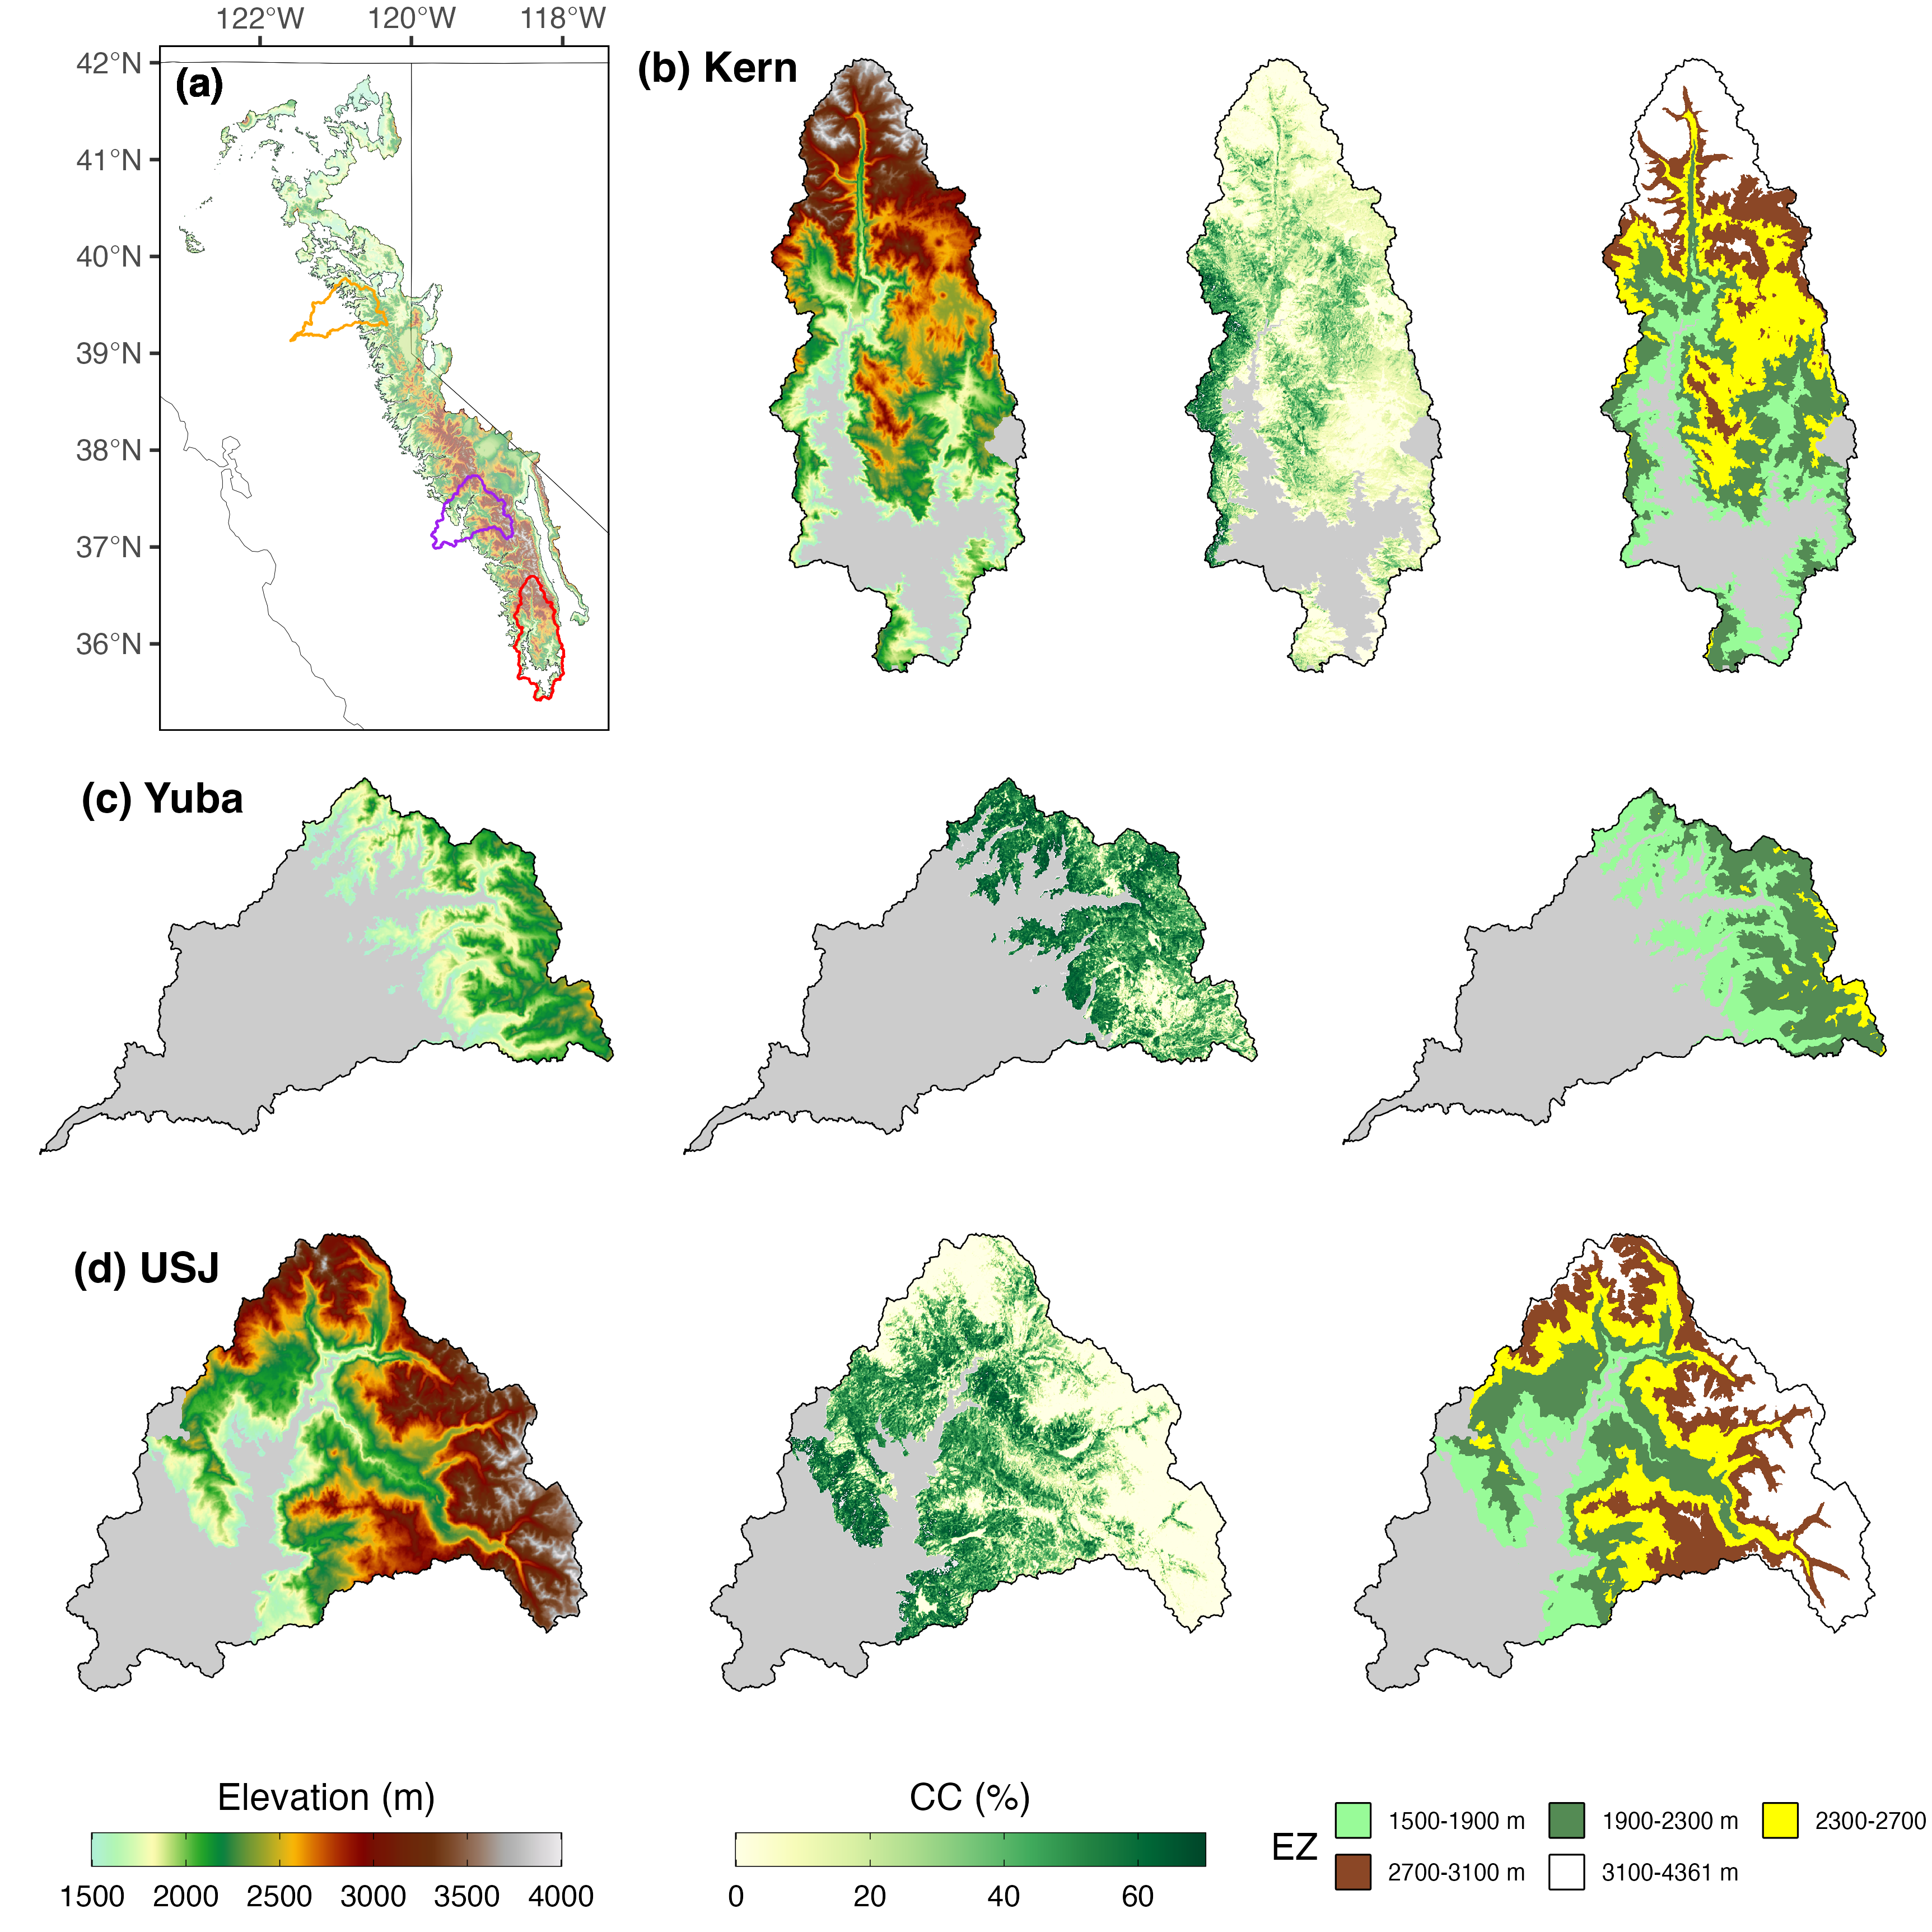
\includegraphics[width=14cm]{figures/ch2_figs/kuy_study_area_v2.png}
\caption{\textbf{(a)} The full extent of the SNSR study domain with Yuba (orange), USJ (purple), and Kern (red) basins shown. From left to right for the \textbf{(b)}~Kern, \textbf{(c)}~Yuba, \textbf{(d)}~USJ: elevation, canopy cover (\%), and elevation zones (EZs).}
\label{kuy_study_area}
\end{figure*}

%f1
\begin{figure*}[t]
\centering
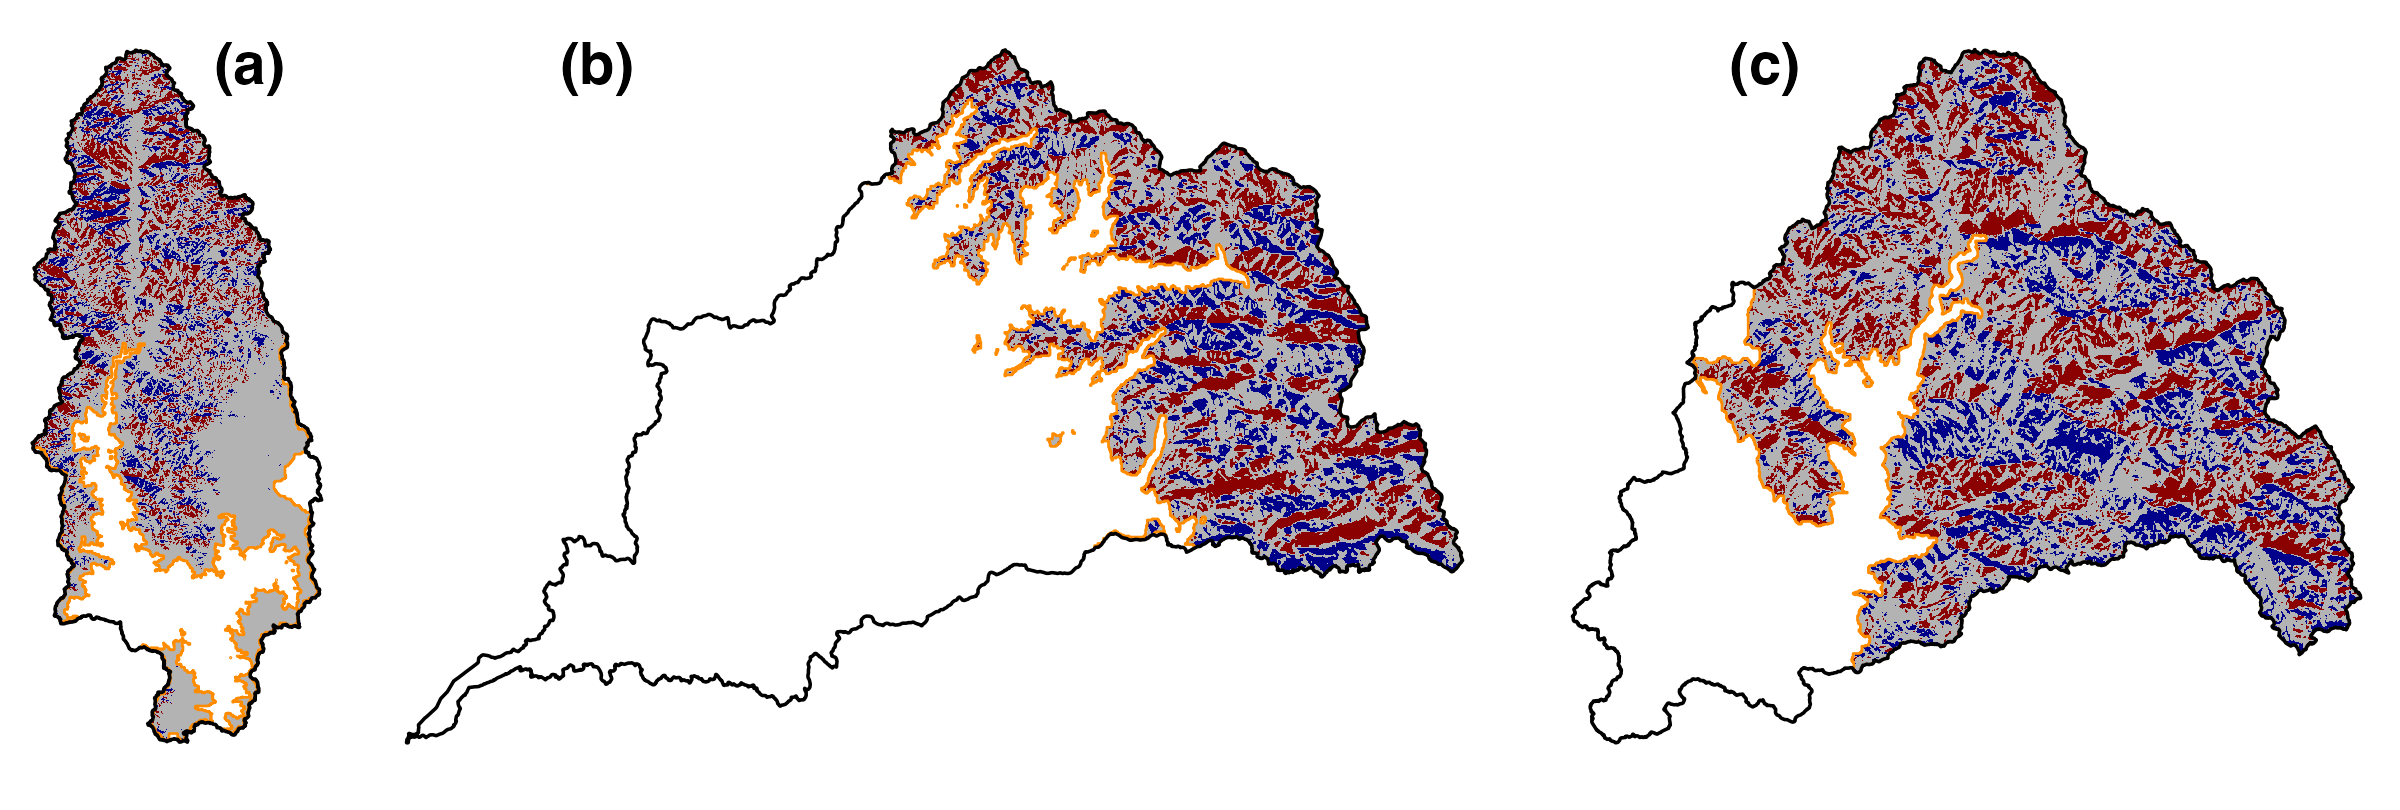
\includegraphics[width=\textwidth]{figures/ch2_figs/kuy_snow_metric_area_v2.png}
\caption{The north (blue) and south (red) facing pixels that met the threshold for inclusion in the study for the \textbf{(a)}~Kern, \textbf{(b)}~Yuba, and \textbf{(c)}~USJ. The orange line is a 1500~m contour, which represents the boundary of the SNSR. The grey area represents pixels in the SNSR modeling domain that are not considered in this study.}
\label{fig:kuy_snow_metric_area}
\end{figure*}



%==============================================================================
\hypertarget{ch2-sa-1}{\subsubsection{Yuba}\label{ch2-sa-1}}

The Yuba River basin is located in the northern Sierra Nevada and is 3483~km$^{2}$ in land area. The Yuba River is the main tributary of the Feather River and eventually runs into the Sacramento River, which is the largest in California. It has the lowest maximum elevation (2713~m) and greatest average canopy cover (42~\%) of the three study basins. 

%==============================================================================
\hypertarget{ch2-sa-2}{\subsubsection{USJ}\label{ch2-sa-2}}

The USJ is approximately 4244~km$^{2}$ in land area, spanning from the high-elevation peaks (4227~m) in the east to flat low-elevation (153~m) Central Valley in the west (Fig.~\ref{fig:multisensor_study_area}). The main channel flows into Millerton Lake, which is one of the largest reservoirs in the Central Valley. 

%==============================================================================
\hypertarget{ch2-sa-3}{\subsubsection{Kern}\label{ch2-sa-3}}

The Kern River basin is the southernmost basin of Sierra Nevada and is 5370~km$^{2}$ in land area. Its southern drainage direction and predominant basin orientation are different that the west-facing Yuba and USJ. It has the greatest maximum elevation (4362~m) --- with the headwaters of the North Fork originating near Mount Whitney --- and the lowest average canopy cover (17~\%) of the three study basins. 

%==============================================================================
%==============================================================================
%==============================================================================
\hypertarget{ch2-do-1}{\subsection{Data Overview}\label{ch2-do-1}}

In this section, we describe the gridded snow reanalysis, meteorologic data, and in situ data used in this study.

%==============================================================================
\hypertarget{ch2-do-2}{\subsubsection{SNSR}\label{ch2-do-2}}

The SNSR \citep{margulisLandsatEraSierraNevada2016} is a 90~m gridded daily SWE product for California Sierra Nevada from water years (WY) 1985--2016. These data were created using a Bayesian particle batch smoother data assimilation (DA) technique to retroactively assimilate Landsat fractional snow-covered area (fSCA) with downscaled National Land Data Assimilation System (NLDAS) meteorological forcings. The MSWE estimates were validated with over 9000 years of snow pillow and snow course data. Detailed information on the development and implementation of this methodology can be found in a series of past publications: \cite{durandBayesianApproachSnow2008, girottoExaminingSpatialTemporal2014, girottoProbabilisticSWEReanalysis2014, margulisParticleBatchSmoother2015}. A recent analysis from \cite{yangIntercomparisonSnowWater2023} evaluated the uncertainty of various SWE products using lidar data from the Airborne Snow Observatories (ASO) \citep{painterAirborneSnowObservatory2016}. They found that the SNSR performed the best according to various error metrics, making it a well-suited data set for our analysis.

\hypertarget{ch2-do-2}{\subsubsection{SNOTEL data}\label{ch2-do-2}}

SWE data from 29 SNOTEL sites totaling $\sim$840 station years (Fig. \ref{kuy_study_area}a) were used for model validation. Operated by the United States Department of Agriculture's Natural Resources Conservation Service (NRCS), it is a comprehensive network of remote, long-term, automated sites spread across the western United States and Alaska. These data are quality controlled by the NRCS.

\hypertarget{ch2-do-2}{\subsubsection{gridMET Data}\label{ch2-do-2}}

We used 4~km meteorological data from gridMET \citep{abatzoglouDevelopmentGriddedSurface2013} to calculate annual (1985--2016) cold season values from October 1 to March 31 (ONDJFM) for three meteorologic variables: mean temperature (T\textsubscript{mean}), relative humidity (RH\textsubscript{mean}), and incoming solar radiation (insolation). Daily ONDJFM where averaged to create the annual metrics. These data were bilinearly downscaled to the 90~m SNSR resolution. Since gridMET does not include a T\textsubscript{mean} or RH\textsubscript{mean} value---only the daily maximum and minimum---these values were averaged to create the two mean variables. Insolation from gridMET is estimated with respect to a planar surface and not topographically corrected. 

%===========================================================================
\hypertarget{ch2-do-2}{\subsubsection{Clear sky insolation}\label{ch2-do-2}}

Clear sky incoming solar radiation (CS insolation) for ONDJFM was estimated using the 90~m spatially distributed mean value. Calculations were performed using the R package “insol” (**cite), which is based on the Bird model \citep{birdReviewEvaluationImprovement1981}. The R insol model uses the SNSR 90~m DEM as input and accounts for slope, aspect, differential shading, day of year, solar zenith angle, air temperature, elevation, and relative humidity. To calculate CS insolation, daily values were averaged in the same fashion as the gridMET data. Note that CS insolation does not account for cloud cover or variations in latitude. Thus, we produce a gridded estimate of CS insolation that represents the average cold-season clear sky radiation for any year (i.e., not a time series).

%==============================================================================
%==============================================================================
%==============================================================================

\hypertarget{ch2-methods-1}{\subsection{Snow metric creation and validation}\label{ch2-methods-1}}

\begin{figure*}[t]
\centering
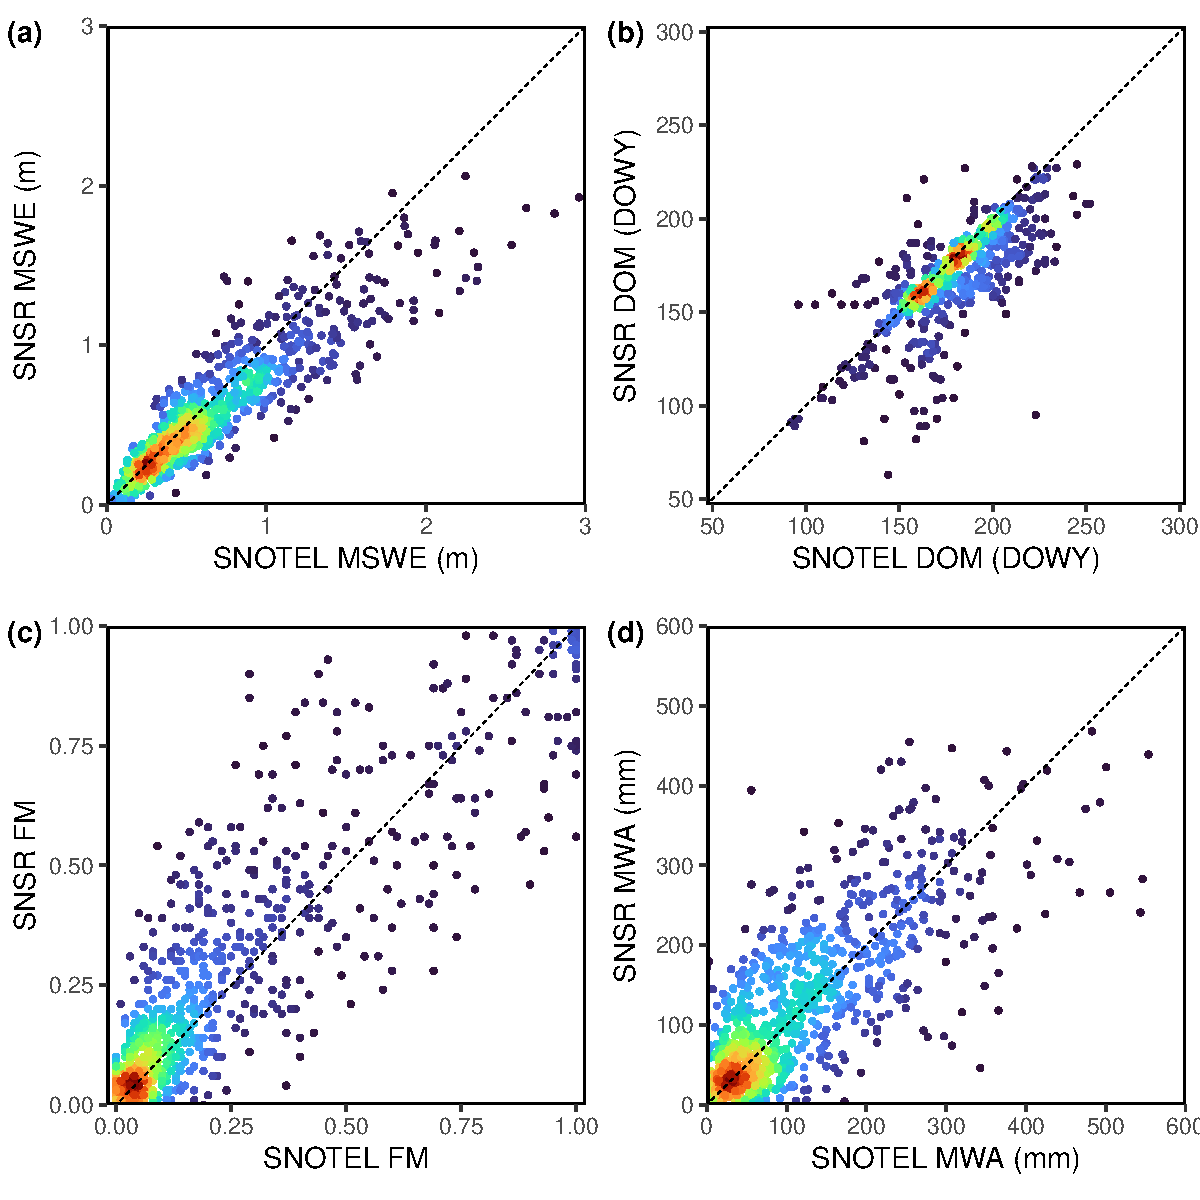
\includegraphics[width=10cm]{figures/ch2_figs/snsr_snotel_metric_compare_new_v1.pdf}
\caption{Density plots comparing SNSR and SNOTEL \textbf{(a)} MSWE, \textbf{(b)} DOM, \textbf{(c)} FM days, \textbf{(d)} MWA for 29 SNOTEL stations from WY 1985--2016 (n $\approx$ 840).}
\label{kuy_study_area}
\end{figure*}

Using the SNSR, we generated four pixel-wise snowpack metrics: MSWE, DOM, FM, and MWA. MSWE is defined as the maximum amount (mm) of SWE in a given pixel for a Water Year (WY, Oct. 1 -- Sept. 30), while DOM is the last day of the water year in which a pixel has that amount. As defined \cite{musselmanWinterMeltTrends2021}, FM is the fraction of ablation (i.e., melt, wind transport, sublimation, evaporation) that occurs before April 1st. MWA is the amount of SWE lost in (mm) during the same time period. Reporting both FM and MWA allows for a more complete understanding of midwinter ablation dynamics, as they provide both a fraction and a magnitude.

We focused our analysis on the seasonal snow zone, which we defined as grid cells that receive at least 26~mm ($\sim$1~in) of SWE for at least 27 of the 32 years in the SNSR data set. While the SNSR data set uses a 1500~m threshold, a preliminary analysis found that many of the lower elevation grid cells, specifically in the Kern, did not contain snow in most years. Fig.~\ref{fig:kuy_snow_metric_area} shows the three basins, the 1500~m SNSR seasonal snow grid cells, and the seasonal north and south-facing snow grid cells considered in this study.

These metrics were then validated against 29 SNOTEL stations totaling $\sim$840 station years (Figure \ref{kuy_study_area}). SNSR values were selected by the specific pixel in which the SNOTEL station fell. Two correlation coefficients (R and R$^{2}$), root-mean-square error (RMSE), mean absolute error (MAE), mean error (ME), and percent bias (PB) are in Table \ref{tab:snow_metrics_val_table}.


\begin{table}[htbp]
  \centering
  \caption{Error statistics (RMSE, MAE, ME, and PB) and correlation coefficients for (R and R$^{2}$) for the MSWE, DOM, and FM compared to 29 SNOTEL stations from WY 1985–-2016 (n $\approx$ 840). The in situ data are compared against the single SNSR pixel in which the station falls.}
  \label{tab:snow_metrics_val_table}
  \begin{tabular}{lrrrrrr}
    \toprule
    Snow Metric & R & R$^{2}$ & RMSE & MAE & ME & PB (\%) \\
    \midrule
    Max SWE (m) & 0.9 & 0.81 & 0.22 & 0.15 & $-$0.08 & $-$11.6 \\
    Max SWE (DOWY) & 0.75 & 0.56 & 18.95 & 11.59 & $-$8.05 & $-$4.5 \\
    FM & 0.88 & 0.77 & 0.14 & 0.09 & 0.03 & 12.5 \\
    MWA (mm) & 0.75 & 0.56 & 71.78 & 52.44 & 9.06 & 7.4 \\
    \bottomrule
  \end{tabular}
\end{table}

\hypertarget{ch2-methods-2}{\subsection{Physiographic disaggregation}\label{ch2-methods-2}}

We disaggregated the basins by their physiographic characteristics (elevation, slope, and aspect) in order to understand the relationship between these physical attributes, snow metrics, and climate. This segmenting also controls for precipitation inputs, where we assume that snowfall amounts are relatively constant throughout the elevation zones (EZs). The basins were segmented into EZs: EZ1 (1500--1900~m), EZ2 (1900--2300~m), EZ3 (2300--2700~m), EZ4 (2700--3100~m), and EZ5 (3100--4361~m). EZ1--4 are split into even 400~m segments, while EZ5 extends from 3100~m to the maximum elevation (4361~m). EZ5 was chosen to be larger to simplify our results, as we found that areas above 3100~m exhibited similar snow metric characteristics. 

The basins were then segmented into north-facing (315--45$^{\circ}$) and south-facing (135--215$^{\circ}$) aspects, with a least a slope of > 4$^{\circ}$ needed to be considered in our analysis. By setting this slope threshold, flatter terrain is excluded, focusing our analysis on complex mountain areas. We did not include east-facing and west-facing slopes in this study. 

\hypertarget{ch2-methods-3}{\subsection{Spearman correlations}\label{ch2-methods-3}}

Spearman's Rho, a non-parametric measure of statistical dependence between variables, was computed to assess the relationship between FM and the three meteorological variables across the EZs and three study basins. The objective of this part of the analysis was to characterize the snow metric sensitivity to the meteorologic data. The analysis was conducted on a pixel-wise basis for the 32-year study period, with each pixel producing $p$ and Spearman's $\rho$ values. As there are $\sim$10$^4$ pixels in each EZ, we calculated the percentage of pixels that displayed significant relationships ($p < .05$).

%==============================================================================
%==============================================================================
%==============================================================================
\hypertarget{ch2-results}{\section{Results}\label{ch2-results}}
\hypertarget{ch2-results-1}{\subsection{Snow metric physiography}\label{ch2-results-1}}

The four snowpack metrics varied significantly, with patterns emerging with respect to basin, elevation, and aspect. The mean values---split into north and south-facing slopes and EZs---of the four snow metrics are displayed in Table \ref{tab:snow_metric_table} with Fig.\ref{fig:snow_boxplots} showing the distributions. We also report the physiographic distribution of the four meteorologic variables in Table \ref{tab:met_metric_table} and Fig. \ref{fig:met_boxplots}.

%f1
\begin{figure*}[t]
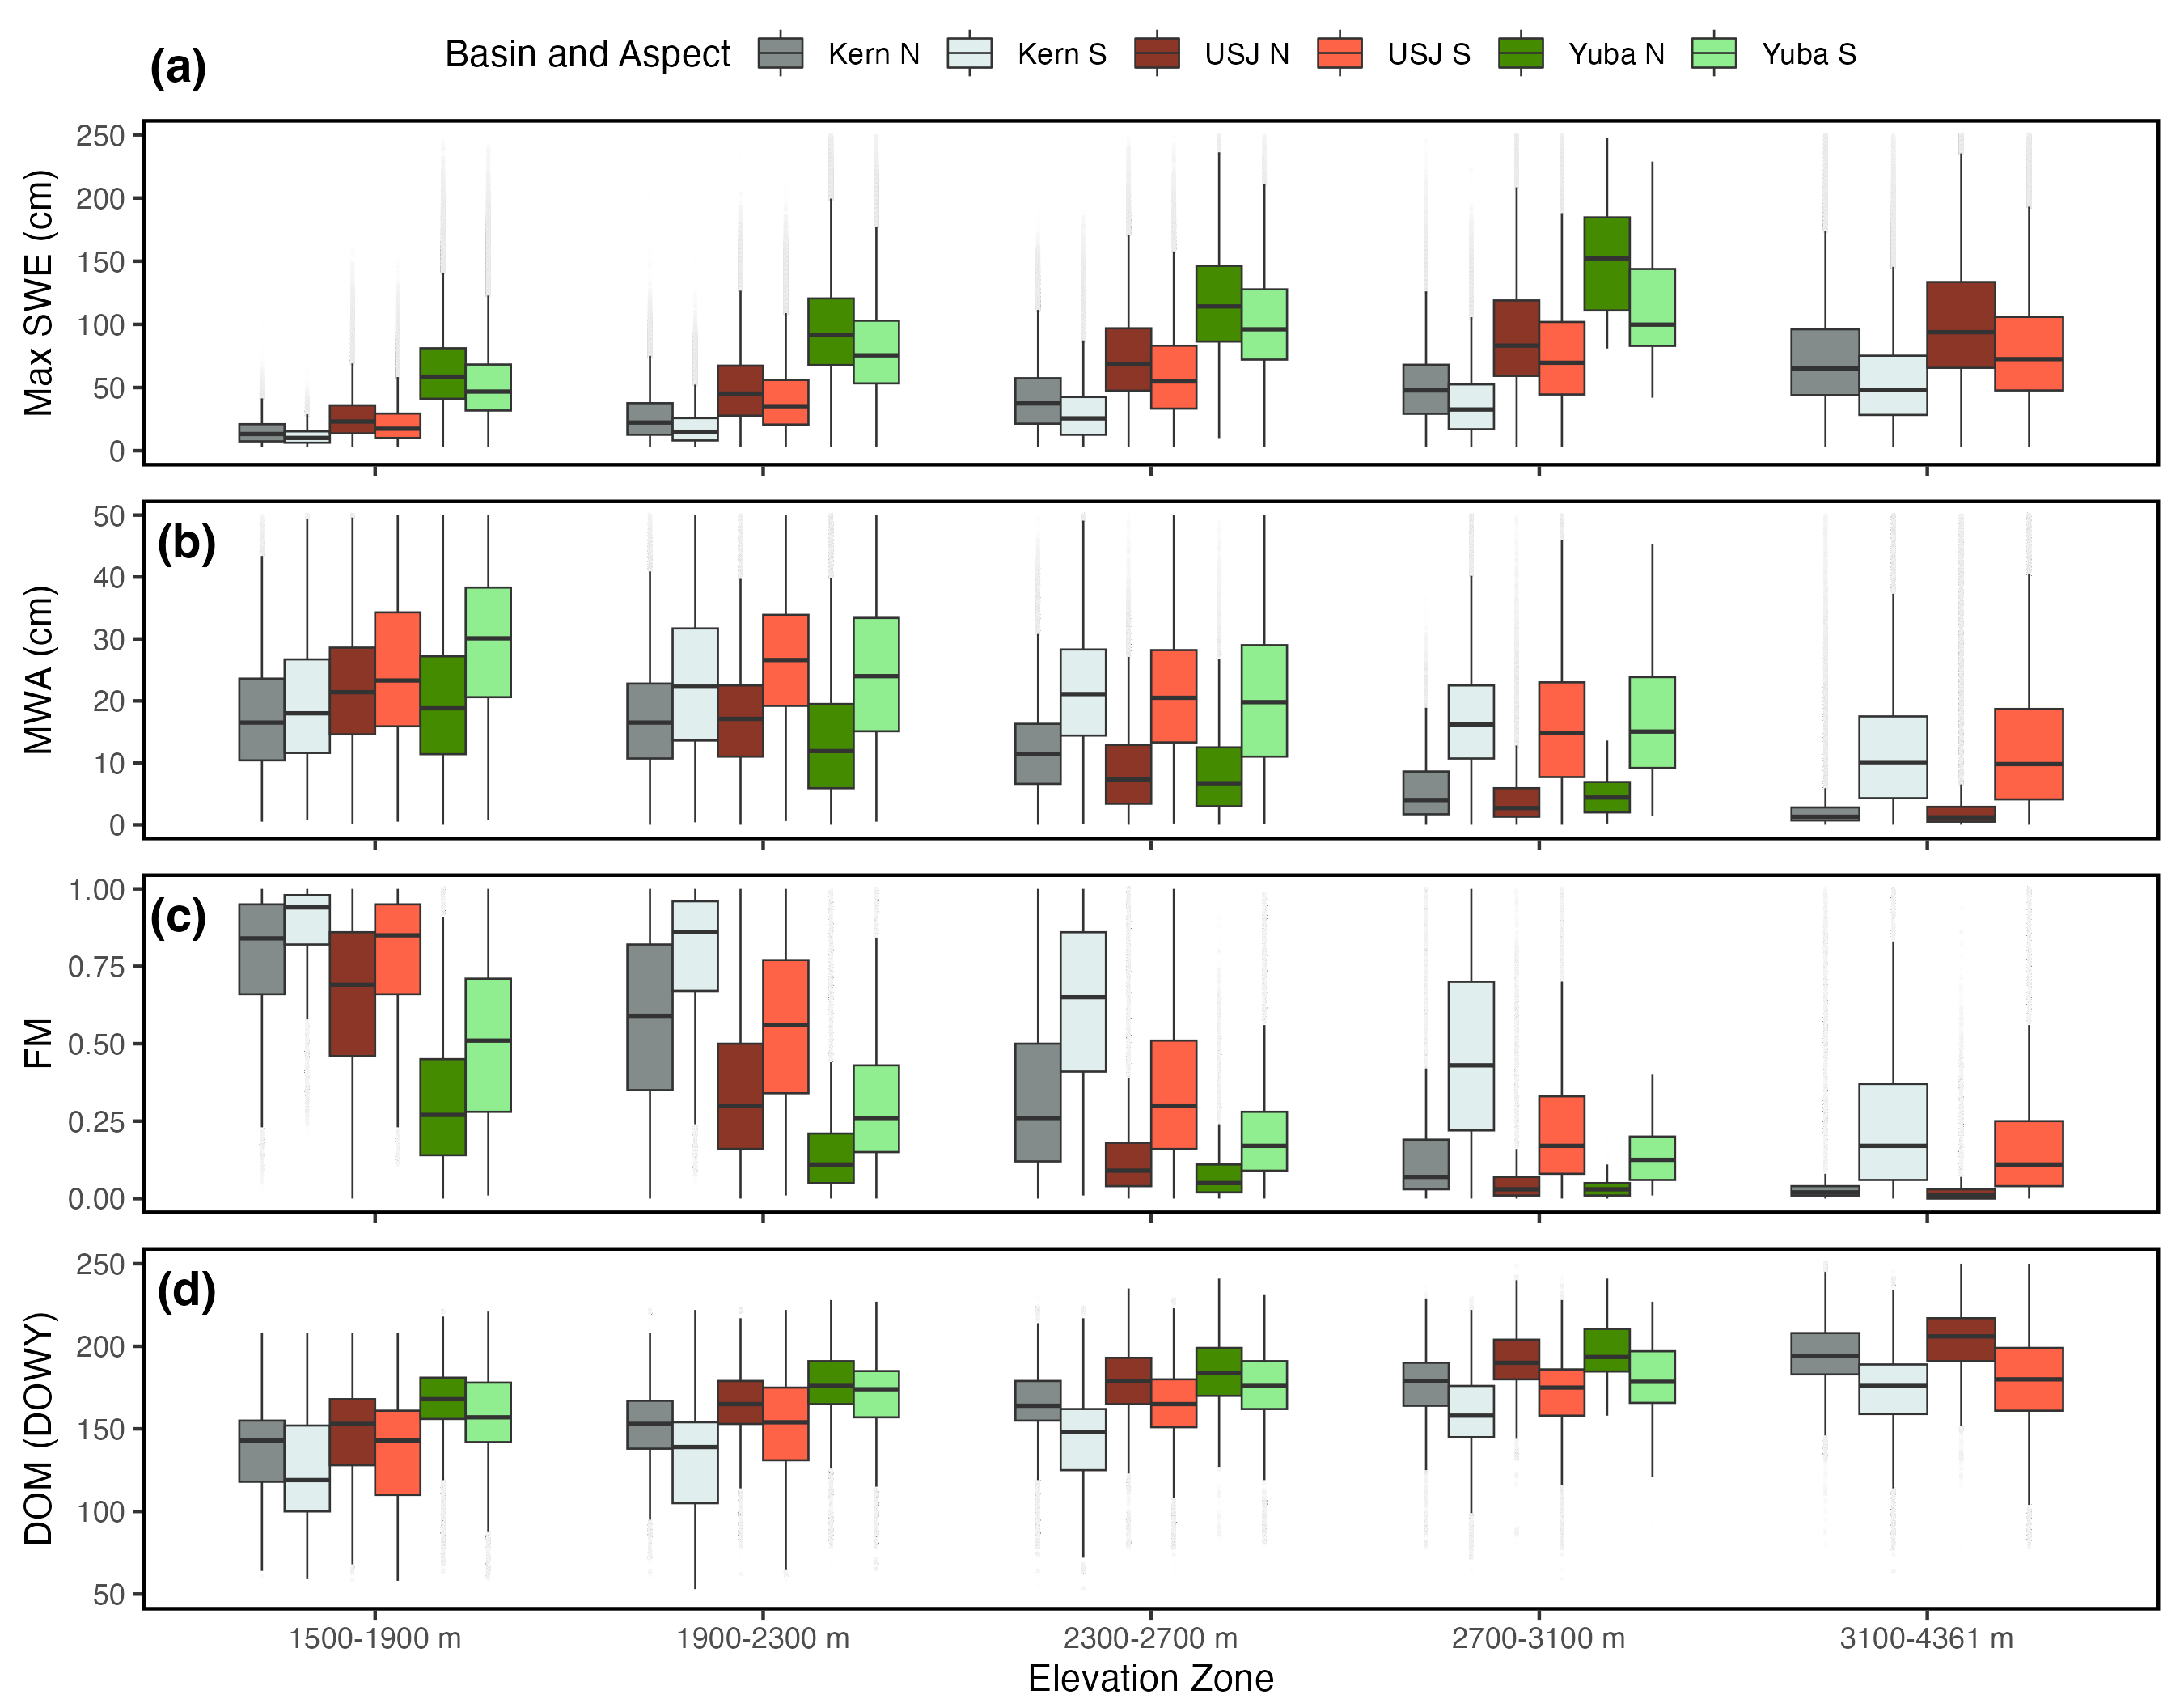
\includegraphics[width=\textwidth]{figures/ch2_figs/snow4_boxplot_v5.png}
\caption{Boxplots for \textbf{(a)} MSWE, \textbf{(b)} MWA, \textbf{(c)} FM, \textbf{(d)} DOM, for the 32-year study period. The data are grouped by the five EZs and colored in the three basins: Kern (gray), USJ (orange), and Yuba (green). The color shading represents north-facing (darker) and south-facing (lighter) slopes for the respective basin.}
\label{fig:snow_boxplots}
\end{figure*}

For all of the snow metrics in all three basins, there are marked differences between the north and south-facing slopes (Fig.~\ref{fig:snow_boxplots}). Overall the Kern, which is the southernmost basin, has the greatest mean FM values (Fig.~\ref{fig:snow_boxplots}a) for all elevation bands when compared to the Yuba and the USJ. Additionally, it had the highest mean FM percent difference between south and north-facing slopes of 69.6~\%. Yet, shown in Fig. \ref{fig:met_boxplots} and Table \ref{tab:met_metric_table}, the Kern has either similar or colder T\textsubscript{mean} values (Fig. \ref{fig:met_boxplots}a) than the Yuba and the USJ. These differences are possibly explained by the insolation values in the Kern (Fig. \ref{fig:snow_boxplots}c) being greater by $\sim$15--25 $\mathrm{W~m}^{-2}$ across all EZs. 

Elevation trends are consistently observed across all three basins for each of the four metrics, although the magnitude of the differences varies incongruently among the basins. As expected, MSWE and DOM increase with elevation, while FM and MWA broadly decrease. The two midwinter ablation metrics (FM and MWA) impact both MSWE and DOM for all basins and EZs. Across the three basins, south-facing slopes reach DOM on average 16.1~d earlier, with the greatest mean difference of 25 d occurring in the USJ between 3100--4361~m. MSWE on north-facing slopes is, on average, 154~mm greater across all basins and EZs. North vs. south-facing disparities are amplified by increasing elevation, with a maximum difference of 467~mm in EZ4 of the Yuba.

For EZ4 (2700--3100~m) and EZ5 (3100--4361~m), the USJ and Kern showed particularly stark differences in both midwinter ablation metrics with respect to aspect. The mean FM and MWA values for the two basins in these EZs on north-facing slopes were 0.07 and 39~mm, respectively. In contrast, south-facing slopes had markedly higher values, with mean FM and MWA values of 0.29 and 151~mm. This means there is approximately 4 times more FM and MWA on south-facing slopes at elevations above 3100~m. We note that T\textsubscript{mean} values are below 0$^{\circ}$ for these areas (\ref{tab:met_metric_table})

Fig.~\ref{fig:aspec_mwa_fm_bp} shows boxplots of T\textsubscript{mean} split into 0.5 C$^{\circ}$ bins plotted against FM (left) and MWA (right) for the three study basins. Across all basins and T\textsubscript{mean} values, south-facing slopes show greater FM and MWA values.  The Kern and USJ have higher elevations, and therefore large areas with cold season T\textsubscript{mean} values below 0~$^{\circ}$C. In the places with T\textsubscript{mean} at or below $-$2~$^{\circ}$C, north-facing slopes show near-zero FM and MWA, while south-facing areas show between 0.15--0.25 and $\sim$100~m, respectively. Broadly, as T\textsubscript{mean} rises, FM and MWA values on north and south-facing slopes become more similar.

For the gridMET derived metrics (T\textsubscript{mean}, RH, insolation), there are no significant differences between the north-facing and south-facing slopes (Figure \ref{fig:met_boxplots}.a--c). This makes sense considering gridMET's native 4~km spatial resolution, thus not capturing the topographic heterogeneity of the 90~m SNSR data. CS insolation shows vast differences in the amount of insolation received by the two aspects. Across all basins and EZs, south-facing slopes have a mean daily value of 234~$\mathrm{W~m}^{-2}$, while north-facing's is 43~$\mathrm{W~m}^{-2}$. Since these are static clear sky estimates, the values say consistent across the three study basins and EZs. However, in the gridMET insolation data, the Kern has the greatest mean basin-wide insolation value of 157~$\mathrm{W~m}^{-2}$. These insolation values decrease as basin latitude increases, with the USJ and Yuba having mean values of 149~$\mathrm{W~m}^{-2}$ and 139~$\mathrm{W~m}^{-2}$, respectively.

\begin{table}[htbp]
\centering
\caption{The mean values of the MWSE, DOM, FM, and FM for the three study basins. Each basin is split into north-facing (NF) and south-facing (SF) with the difference between the two also shown.}
\label{tab:snow_metric_table}
\tiny % Reduce font size to \small
\begin{tabular}{llrrrrrrrrrrrr}
\toprule
& & \multicolumn{3}{c}{MSWE (mm)} & \multicolumn{3}{c}{DOM (DOWY)} & \multicolumn{3}{c}{FM} & \multicolumn{3}{c}{MWA (mm)} \\
\midrule
Basin & EZ & NF & SF & Diff & NF & SF & Diff & NF & SF & Diff & NF & SF & Diff \\
\midrule
Kern & 1500--1900 m & 151 & 116 & $-$35 & 138 & 127 & $-$11 & 0.78 & 0.87 & 0.09 & 178 & 201 & 23 \\
Kern & 1900--2300 m & 269 & 191 & $-$78 & 149 & 133 & $-$16 & 0.58 & 0.79 & 0.21 & 171 & 238 & 67 \\
Kern & 2300--2700 m & 414 & 301 & $-$113 & 164 & 143 & $-$21 & 0.34 & 0.62 & 0.28 & 119 & 222 & 103 \\
Kern & 2700--3100 m & 518 & 375 & $-$143 & 178 & 156 & $-$22 & 0.15 & 0.47 & 0.32 & 56 & 177 & 121 \\
Kern & 3100--4361 m & 744 & 555 & $-$189 & 195 & 173 & $-$22 & 0.04 & 0.25 & 0.21 & 25 & 123 & 98 \\
USJ & 1500--1900 m & 267 & 219 & $-$48 & 146 & 136 & $-$10 & 0.65 & 0.78 & 0.13 & 218 & 262 & 44 \\
USJ & 1900--2300 m & 505 & 411 & $-$94 & 163 & 149 & $-$14 & 0.35 & 0.56 & 0.21 & 172 & 282 & 110 \\
USJ & 2300--2700 m & 745 & 614 & $-$131 & 178 & 162 & $-$16 & 0.14 & 0.35 & 0.21 & 87 & 221 & 134 \\
USJ & 2700--3100 m & 927 & 771 & $-$156 & 191 & 172 & $-$19 & 0.06 & 0.24 & 0.18 & 43 & 170 & 127 \\
USJ & 3100--4361 m & 1068 & 808 & $-$260 & 204 & 179 & $-$25 & 0.03 & 0.18 & 0.15 & 31 & 133 & 102 \\
Yuba & 1500--1900 m & 637 & 531 & $-$106 & 166 & 153 & $-$13 & 0.31 & 0.5 & 0.19 & 203 & 335 & 132 \\
Yuba & 1900--2300 m & 960 & 809 & $-$151 & 176 & 168 & $-$8 & 0.15 & 0.31 & 0.16 & 136 & 272 & 136 \\
Yuba & 2300--2700 m & 1210 & 1020 & $-$190 & 184 & 174 & $-$10 & 0.08 & 0.21 & 0.13 & 85 & 221 & 136 \\
Yuba & 2700--3100 m & 1660 & 1193 & $-$467 & 196 & 178 & $-$18 & 0.04 & 0.15 & 0.11 & 61 & 178 & 117 \\
\bottomrule
\end{tabular}
\end{table}


\begin{figure*}[t]
\centering
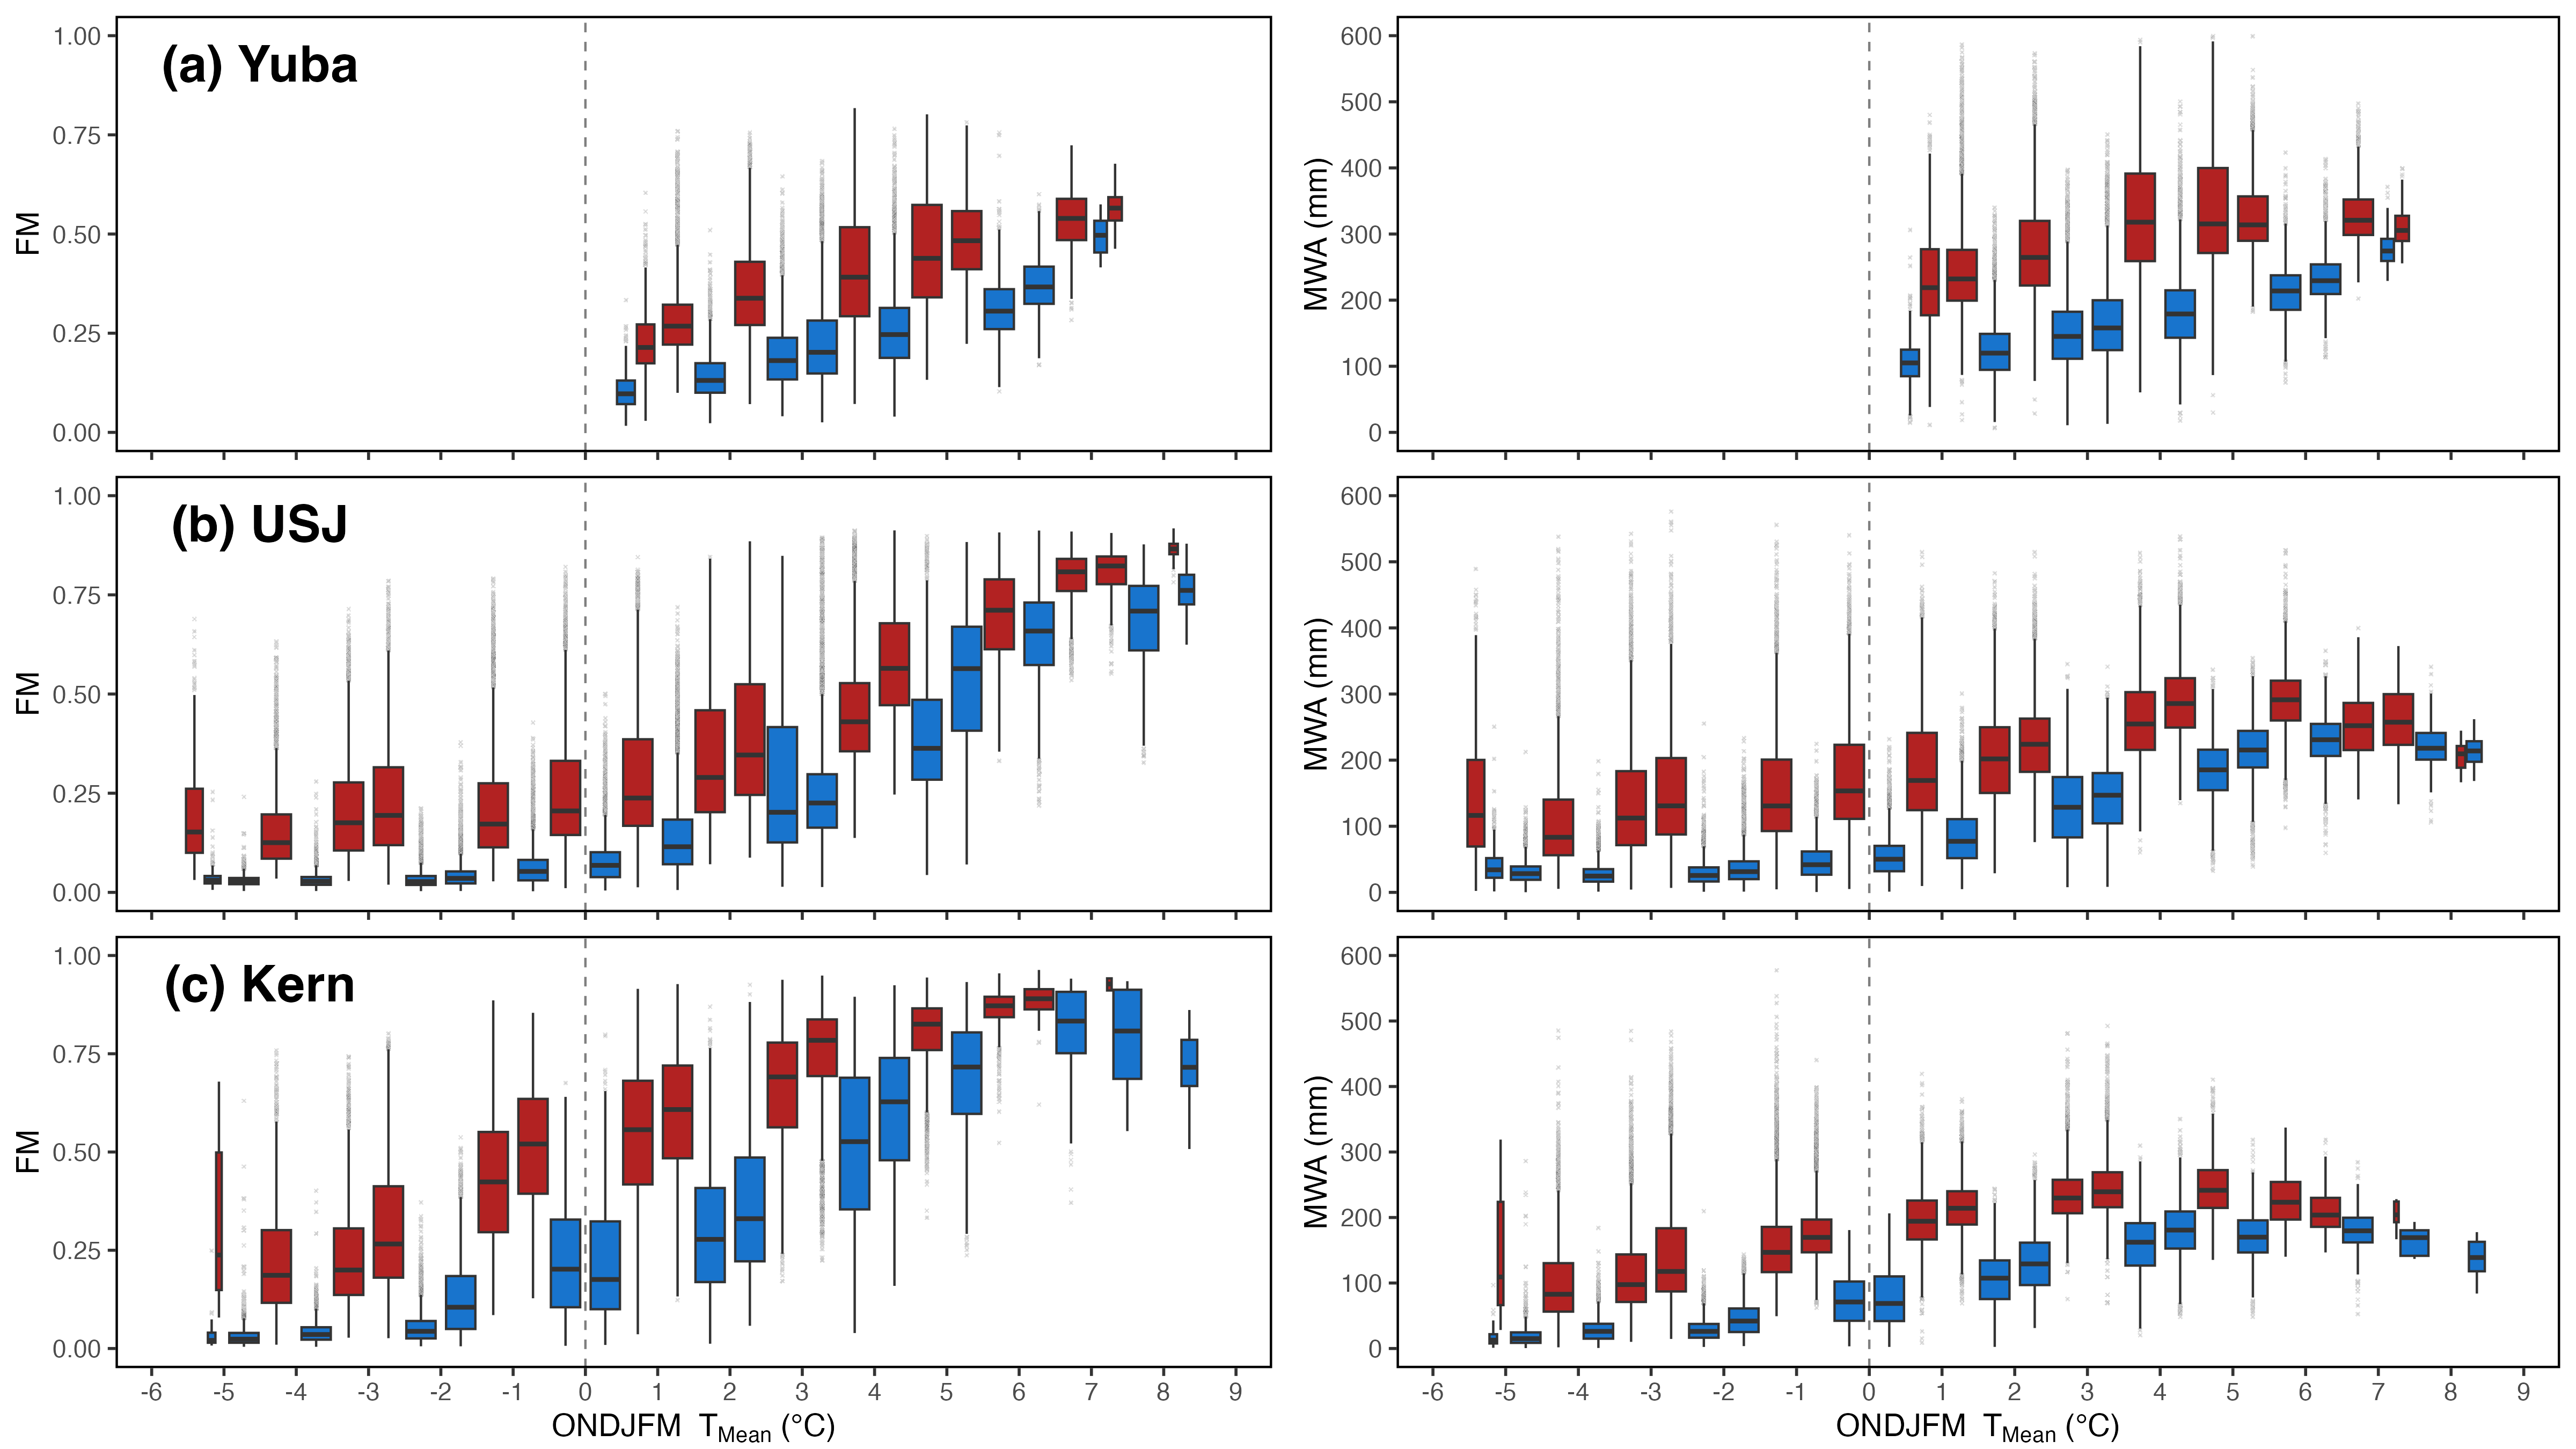
\includegraphics[width=\textwidth]{figures/ch2_figs/aspect_temp_mwa_fum_full_boxplots_v2.png}
\caption{Boxplots comparing FM (left) and MWA (right) on north-facing (blue) and south-facing (red) slopes for the \textbf{(a)} Yuba, \textbf{(b)} USJ, \textbf{(c)} Kern.}
\label{fig:aspec_mwa_fm_bp}
\end{figure*}

\begin{figure*}[h]
\centering
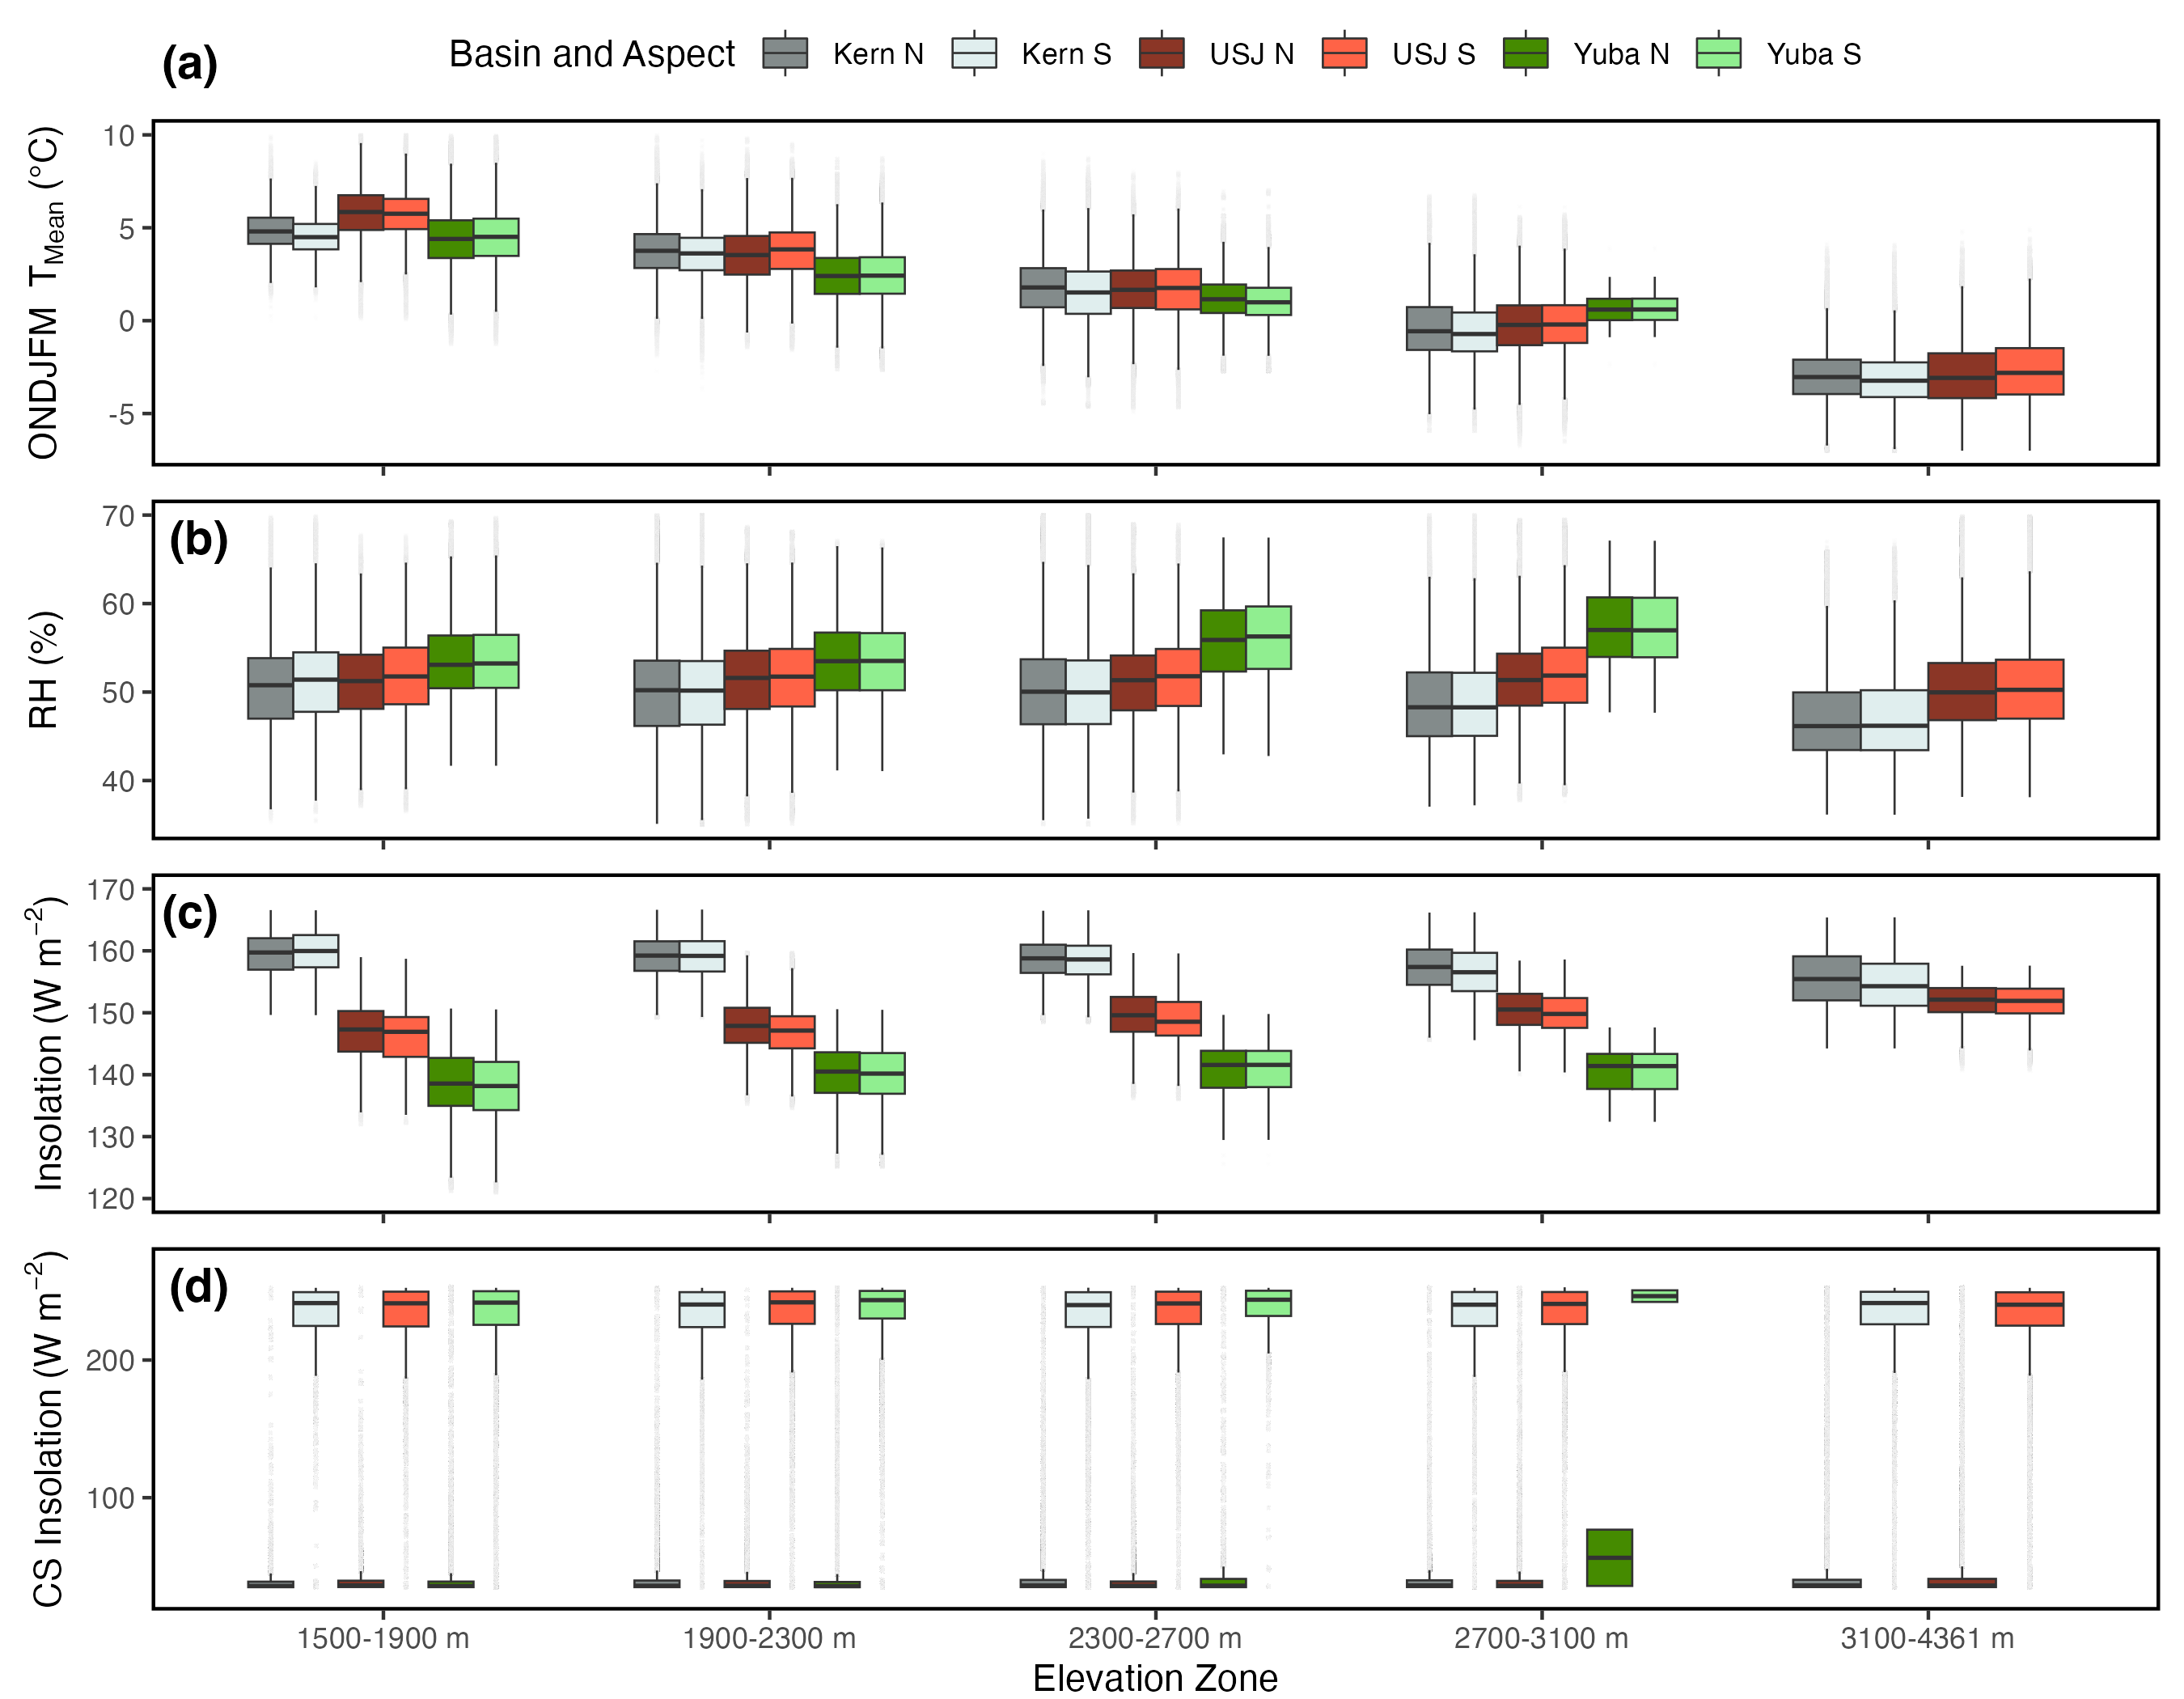
\includegraphics[width=\textwidth]{figures/ch2_figs/met4_boxplot_v5.png}
\caption{Boxplots for \textbf{(a)} T\textsubscript{mean}, \textbf{(b)} RH, \textbf{(c)} insolation, and \textbf{(d)} CS insolation for the 32-year study period. The data are grouped by the five EZs and colored the three basins: Kern (gray), USJ (orange), Yuba (green). The colors shading represents north-facing (darker) and south-facing (lighter) slopes for the respective basin.}
\label{fig:met_boxplots}
\end{figure*}

\begin{table}[htbp]
\centering
\caption{The mean values of the T\textsubscript{mean}, RH, insolation, and CS insolation for the three study basins. Each basin is split into north-facing (NF) and south-facing (SF) with the difference between the two also shown.}
\label{tab:met_metric_table}
\tiny 
\begin{tabular}{llrrrrrrrrrrrr}
\toprule
& & \multicolumn{3}{c}{T\textsubscript{mean} ($^{\circ}$)} & \multicolumn{3}{c}{RH (\%)} & \multicolumn{3}{c}{Insolation ($\mathrm{W~m}^{-2}$)} & \multicolumn{3}{c}{CS Insolation ($\mathrm{W~m}^{-2}$)} \\
\midrule
Basin & EZ & NF & SF & Diff & NF & SF & Diff & NF & SF & Diff & NF & SF & Diff \\
\midrule
    Kern & 1500--1900 m & 4.98 & 4.68 & $-$0.3 & 50 & 51 & 1 & 159 & 159 & 0 & 41 & 231 & 190 \\
    Kern & 1900--2300 m & 3.86 & 3.68 & $-$0.18 & 50 & 50 & 0 & 159 & 158 & $-$1 & 41 & 232 & 191 \\
    Kern & 2300--2700 m & 1.83 & 1.56 & $-$0.27 & 50 & 50 & 0 & 158 & 158 & 0 & 41 & 232 & 191 \\
    Kern & 2700--3100 m & $-$0.39 & $-$0.55 & $-$0.16 & 49 & 49 & 0 & 157 & 156 & $-$1 & 41 & 233 & 192 \\
    Kern & 3100--4361 m & $-$2.98 & $-$3.13 & $-$0.15 & 47 & 47 & 0 & 155 & 154 & $-$1 & 46 & 233 & 187 \\
    USJ & 1500--1900 m & 5.83 & 5.78 & $-$0.05 & 51 & 52 & 1 & 147 & 146 & $-$1 & 40 & 232 & 192 \\
    USJ & 1900--2300 m & 3.56 & 3.78 & 0.22 & 52 & 52 & 0 & 147 & 147 & 0 & 39 & 233 & 194 \\
    USJ & 2300--2700 m & 1.64 & 1.68 & 0.04 & 51 & 52 & 1 & 149 & 148 & $-$1 & 40 & 234 & 194 \\
    USJ & 2700--3100 m & $-$0.28 & $-$0.2 & 0.08 & 52 & 52 & 0 & 150 & 149 & $-$1 & 41 & 233 & 192 \\
    USJ & 3100--4361 m & $-$2.92 & $-$2.7 & 0.22 & 50 & 51 & 1 & 151 & 151 & 0 & 46 & 232 & 186 \\
    Yuba & 1500--1900 m & 4.42 & 4.52 & 0.1 & 53 & 53 & 0 & 138 & 137 & $-$1 & 41 & 231 & 190 \\
    Yuba & 1900--2300 m & 2.45 & 2.47 & 0.02 & 54 & 54 & 0 & 140 & 140 & 0 & 41 & 236 & 195 \\
    Yuba & 2300--2700 m & 1.22 & 1.09 & $-$0.13 & 56 & 56 & 0 & 140 & 140 & 0 & 47 & 236 & 189 \\
    Yuba & 2700--3100 m & 0.69 & 0.7 & 0.01 & 57 & 57 & 0 & 140 & 140 & 0 & 56 & 246 & 190 \\
\bottomrule
\end{tabular}
\end{table}




\hypertarget{ch2-results-3}{\subsection{Snow metric climate sensitivity}\label{ch2-results-3}}

Fig.~\ref{fig:heat_map} displays the results of our Spearman correlations between FM on north and south-facing slopes three meteorological variables: T\textsubscript{mean}, RH, and insolation. Overall the Yuba is the most sensitive basin, as FM is highly sensitive to the three variables tested on both south-facing slopes in all EZs. For the three lowest EZs, spanning 1500--3100~m, a minimum of 90~\% of the land area shows significant relationships between FM and T\textsubscript{mean}. 

The Kern and the USJ display similar patterns for the various correlations; therefore, we group these basins together when reporting their results below. For the top two EZs (2700--4361~m) in the Kern and USJ, the T\textsubscript{mean} sensitivity on north and south-facing slopes diverge. Seen on the right side of Fig.~\ref{fig:heat_map}, the USJ and Kern have a north-facing mean of 14.5~\% of the area that is temperature sensitive, while south-facing slopes show a markedly greater mean value of 70~\%. In contrast, this relationship reverses for the EZ1 and EZ2, where north-facing slopes have a greater mean sensitive area (96~\%) while south-facing slopes show much less significance (mean of 65 \%). We note that the low percentage areas of significant relationship in EZ1--2 does not mean low FM---these areas have the largest mean FM values of anywhere in the study---it just means the FM wasn't correlated to T\textsubscript{mean}.

-report results for RH and insolation...


\begin{figure*}[h]
\centering
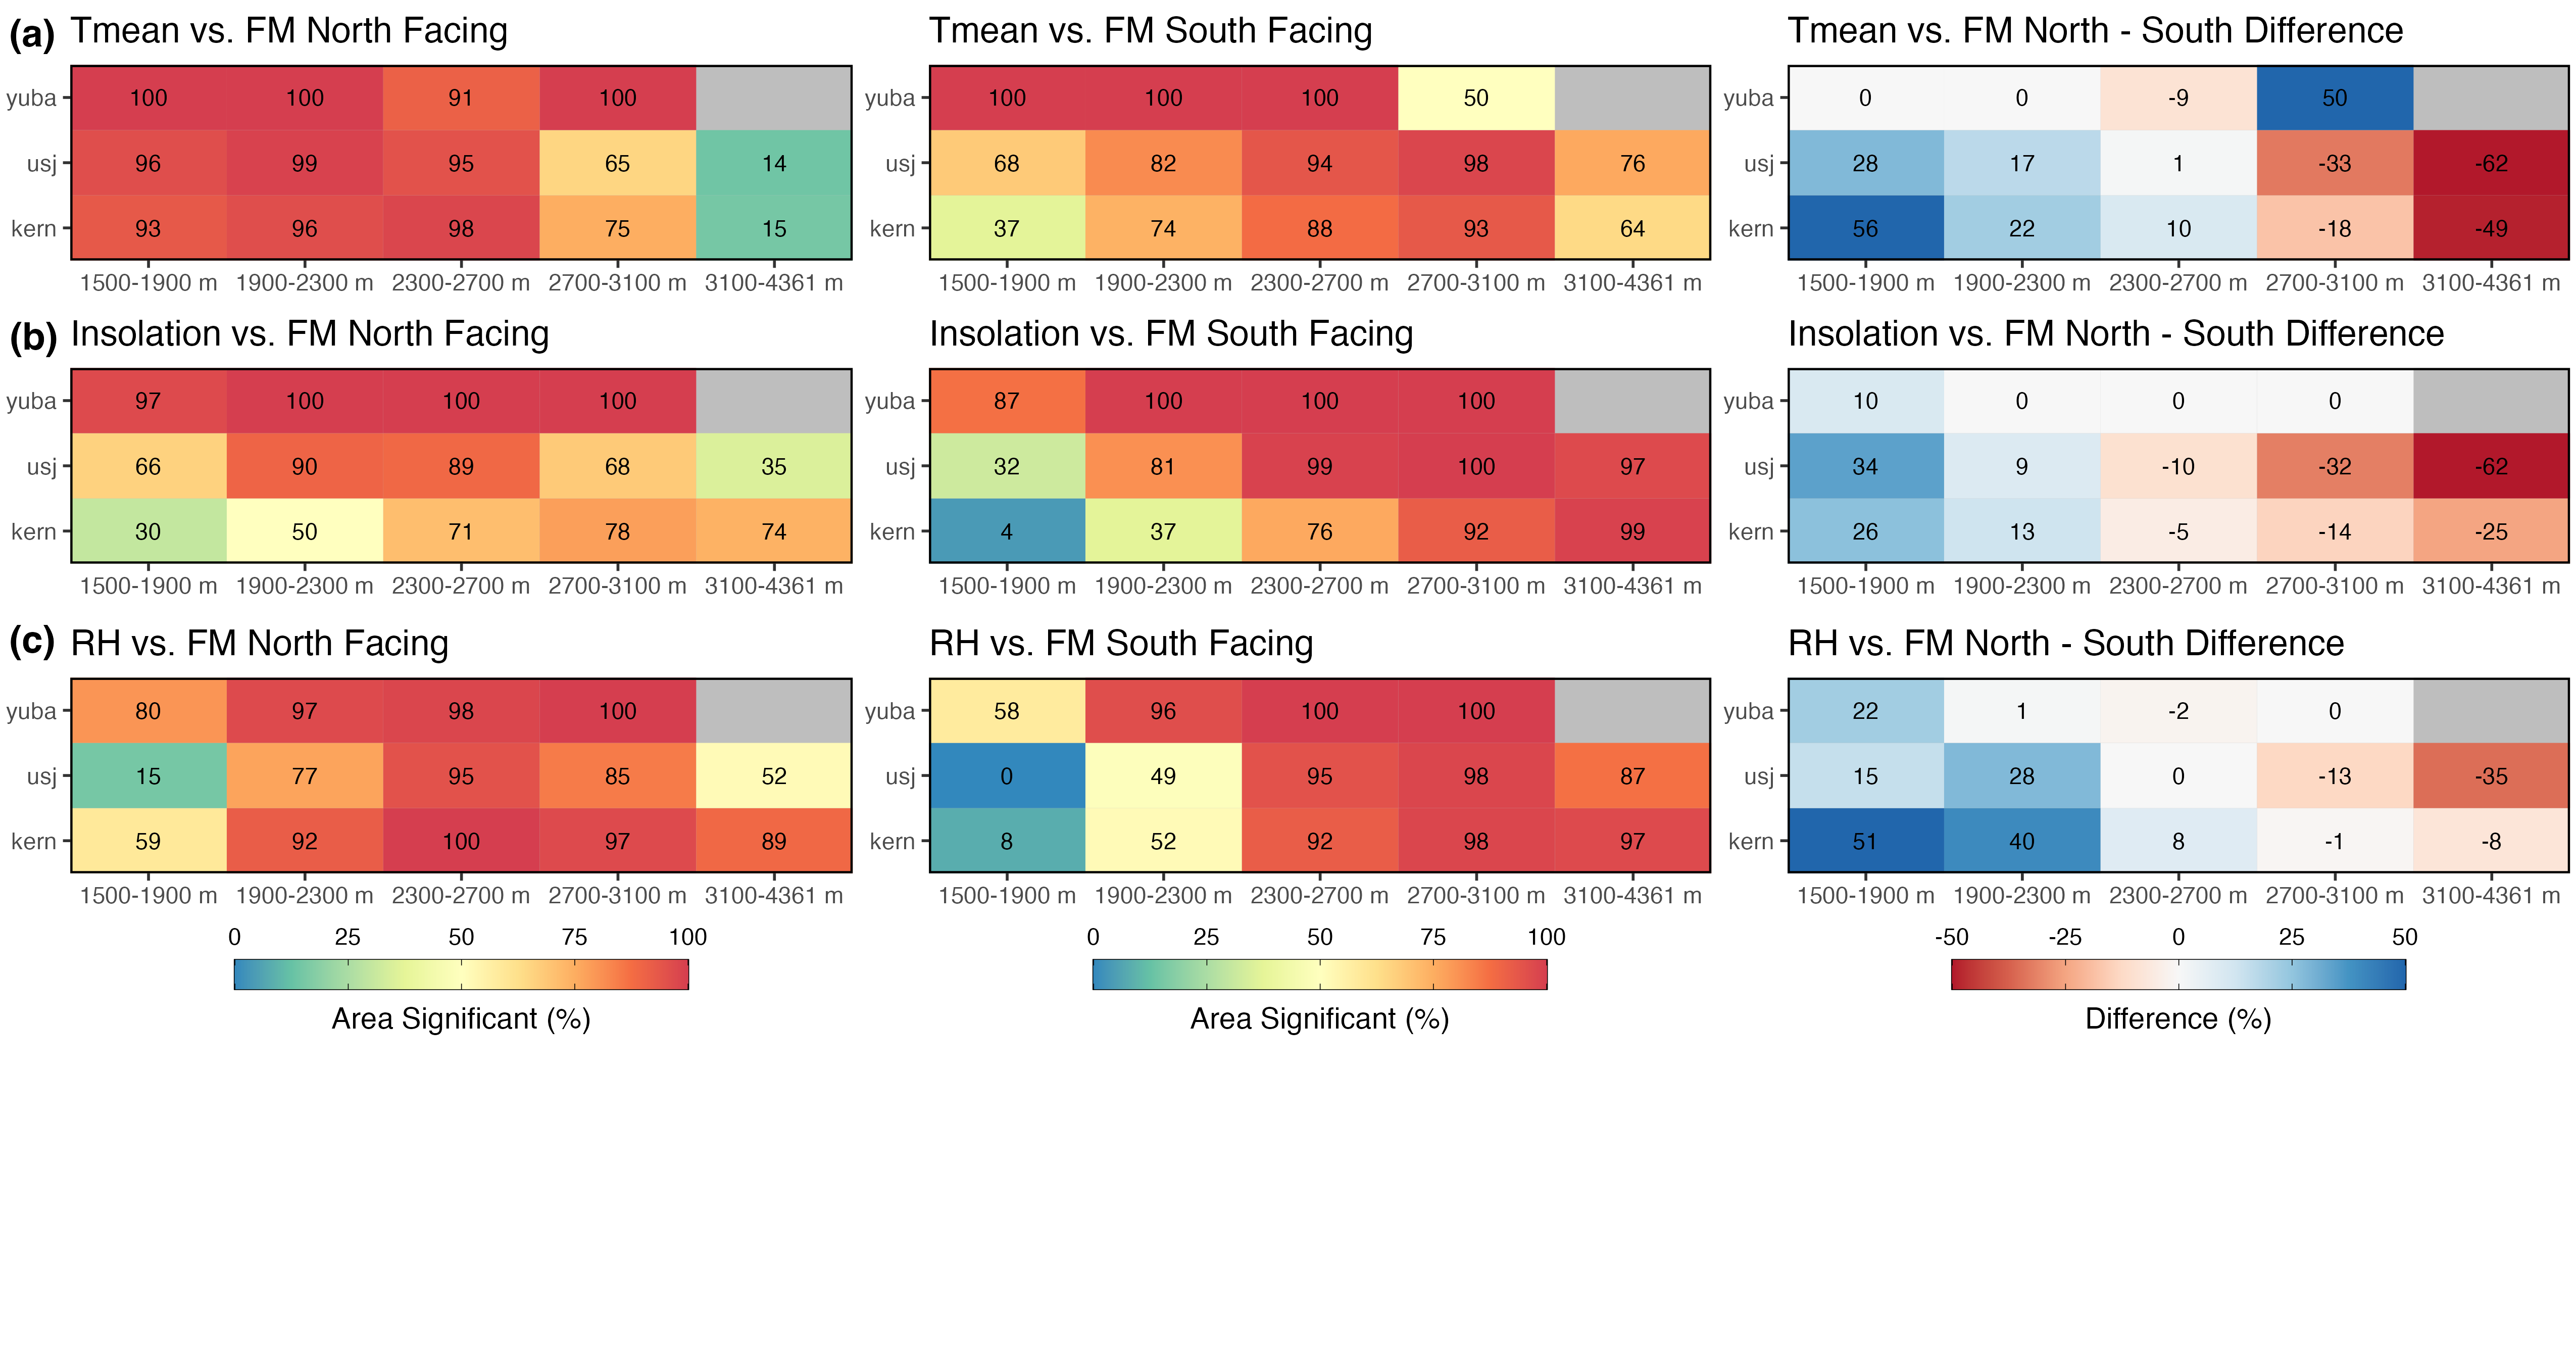
\includegraphics[width=\textwidth]{figures/ch2_figs/metvars_fm_heatmaps_v4.png}
\caption{Heat maps of the displaying percentage of area in each EZ with significant trends ($p < .05$) for \textbf{(a)} T\textsubscript{mean}, \textbf{(b)} RH, and \textbf{(c)} insolation for the 32-year study period. The panels are split into north (left), south-facing (center) slopes, and the difference between the two (right). The color bars correspond to the values within a given panel. Elevation in the Yuba does not rise above 3100~m, shown by a gray value in the heatmap.}
\label{fig:heat_map}
\end{figure*}



%==============================================================================
%==============================================================================
%==============================================================================
\hypertarget{ch2-discussion}{\section{Discussion}\label{ch2-discussion}}
\hypertarget{ch2-discussion}{\subsection{Key findings}\label{ch2-discussion}}


This study has quantified aspect-driven midwinter ablation variations with respect to T\textsubscript{mean} and elevation. We showed that FM and MWA are highly spatially variable, with significant differences emerging with respect to aspects across all EZs. We also showed that midwinter ablation impacts propagate into the MSWE and DOM values, making the spatial quantification of these metrics important for seasonal water resource forecasting. The lower elevation areas showed the greatest midwinter ablation, with these areas having vastly more land area than the higher elevation alpine zones.

- add info on climate sensitivity...

These snowpack processes are extremely variable across rugged mountain topography, and unless they are disaggregated by physiographic characteristics, we have an incomplete understanding of key snow metrics. Station-based snowpack measurements on relatively flat terrain are unable to characterize this hydrologically-important spatial variability. Thus, study provides the first quantified understanding of physiographic impacts on mid-winter ablation in three climatologically-sensitive snow-dominated basins. 


\hypertarget{ch2-discussion}{\subsection{Thoughts on physical mechanisms}\label{ch2-discussion}}

While this study focused on quantifying relationships, it can begin to offer insights into possible physical mechanisms for the documented variability.
The snow metric spatial variability is driven by snowpack cold content. Before we can have any melt, all cold content must be removed from the snowpack. The primary control on snowpack cold content is the amount and temperature of snowfall \citep{jenningsObservationsSimulationsSeasonal2018}, with a negative energy balance being a secondary control. Areas at high elevations (EZ4--5) have a greater amount of snowpack cold content as a result of greater total season snowfall and colder snowpacks. These two factors make the high-elevation snowpack, especially north-facing slopes, less sensitive to warming temperatures. The Spearman correlations further support these findings, with high-elevation north-facing slopes showing limited temperature sensitivity. This suggests that these areas, due to their higher snowpack cold content and lower overall energy inputs, will be less sensitive to warmer temperatures. We hypothesize north-facing high-elevations areas aren't sensitive to sensible heat driven midwinter ablation for two reasons; T\textsubscript{mean} rises above 0~$^{\circ}$C less frequently, and when it does, the sensible heat flux contributes to decreasing cold content rather than snow ablation. In contrast, we showed that south-facing slopes at these higher elevations have, on average, four times greater FM and MWA. This indicates that insolation is a driving factor in high-elevation midwinter ablation as it is the only meteorological factor that varies significantly with respect to aspect. Conversely, the warmest T\textsubscript{mean} values have the most similar north and south-facing values for the midwinter ablation metrics (Fig.~\ref{fig:snow_boxplots}). This implies that at these warmer temperatures---which are low-elevation, shallower, and lower cold content snowpacks---sensible heat flux is driving the melt and sublimation. 

%%%% 




At lower elevations, warmer snowpack temperatures lead to greater snow grain metamorphism and larger grain sizes \citep{colbeckOverviewSeasonalSnow1982}. This leads to a secondary, amplifying effect: greater absorption of solar radiation in the near-infrared wavelengths by larger snow grains \citep{wiscombeModelSpectralAlbedo1980, warrenModelSpectralAlbedo1980}. Moreover, midwinter ablation will increase the concentration of light-absorbing impurities on the snowpack surface (hatchett, gleason, skiles/painter). In the Sierra Nevada, Hatchett et al. document the increase in frequency and length of mid winter dry spells and their interactions with post-fire black carbon on snowpacks in burned forests. 

%%%  forest
While not explicitly included in this study, forest structure and composition affect snowpack accumulation and ablation. \cite{rothForestImpactsSnow2017} and \cite{lundquistLowerForestDensity2013} have shown that snowpacks in warmer, lower-elevation forests melt earlier than those in colder, higher elevations. However, they did not evaluate the effects of slope and aspect on differential snowmelt process. \cite{pelletierWhichWayYou2018a} states that aspect is a key control on forest structure and composition. As shown by our CS insolation model, south-facing slopes receive $\sim$191 $\mathrm{W~m}^{-2}$ more direct solar radiation. Solar radiation is a primary driver for evaporation and sublimation at both the snow and soil surfaces (CITE), impacting plant available water, and therefore decreasing vegetation biomass on south-facing slopes \citep{zapata-riosInfluenceTerrainAspect2016}. Lower forest density allows more insolation to reach the snow surface. There are strong linkages and feedbacks among aspect, insolation, forest cover, and snow hydrology. However, when considering other energy balance components, forest-snow interactions are more complicated.  A comprehensive evaluation of forest impacts on snow across north and south-facing aspects is beyond the scope of this study.

\hypertarget{ch2-discussion-1}{\subsection{Limitations and future work}\label{ch2-discussion-1}}

% model validation 
For the validation of the modeled snow metrics, our study utilized 29 SNOTEL stations, primarily centered around Lake Tahoe. We did not include the California Department of Water Resources (CADWR) snow pillows, as they have known data consistency issues. Future work should implement a quality-controlled version of these data into any model validation, as their geographic range is a better representation of the entire Sierra. While in situ station-based measurements are physiographically limited, they are the best available data source for large-scale model validation. Advancing our understanding of mountain snow hydrology will require synergistic use of in situ data, gridded snowpack energy balance models, and high-resolution satellite remote sensing of various snowpack properties (e.g., SWE, snow depth) \citep{flemingSNOTELSoilClimate2023}.

% temperature uncertainties
There are a number of uncertainties in this analysis. Temperature uncertainties stem from the relatively coarse, 4~km spatial scale of the gridMET data, which may not represent complex microclimates and aspect-driven variation in insolation or temperature. Previous work indicates that temperature patterns and lapse rates vary at relatively fine spatial scales \citep{lundquistSurfaceTemperaturePatterns2007, robledanoModellingSurfaceTemperature2022}, but these variations were not accounted for in our analysis. Future work could implement the 800~m PRISM (Parameter-elevation Relationships on Independent Slopes Model) data \citep{dalyStatisticalTopographicModelMapping1994} or thermal remote sensing data (e.g., Huntingon, lundquist) for finer spatial resolution. The gridMET insolation data show temperature trends in both elevation and latitude. Our CS insolation model does not account for these variations, and adding this variability should be considered for future work.

%% wind and slopes
A second source of uncertainty is via wind redistribution of snow, which substantially affects the snowpack spatial variability in the form of such features as snow dunes, cornices, and sastrugi *** \citep{winstralSpatialSnowModeling2002,marksSimulationTerrainForest2002}.  Wind redistribution of snow is not specifically parameterized in the SNSR. Depending on the prevailing wind direction (westerly in the Sierra), lee-facing slopes tend to have deeper snowpack than scoured windward slopes. We were interested in investigating the relationships between radiation, temperature, and midwinter ablation, therefore omitted east and west-facing slopes from our analysis.

%% forest
Differences in forest cover over time are not considered in the SNSR data set and thus, not part of this study. The SNSR uses a static land cover representation based on the National Land Cover Database (NLCD) \citep{homerConterminousUnitedStates2020}. This does not account for large-scale forest disturbances, mainly forest fires in the Sierra, which are increasing in both area and intensity in the seasonal snow zone \citep{koshkinWildfireImpactsWestern2022}. Future large-scale snow modeling work should look to implement temporally variable land cover characteristics, as forest fires have a significant impact on snow albedo \cite{gleasonCharredForestsIncrease2013} and the timing and magnitude of water resources \citep{williamsGrowingImpactWildfire2022}.

%% geogrpahy
Another consideration is the geographic representativeness of the study basins. We analyzed two west-facing basins (Yuba and USJ) and one south-facing basin in the Sierra. They may not encapsulate the full geographic and physiographic diversity of the range. We used subjective cut-offs for north-facing (315--45$^{\circ}$) vs. south-facing (135--215$^{\circ}$) aspects and for what is considered a slope (> 4$^{\circ}$).

%=============================================================================
%=============================================================================
%=============================================================================
\hypertarget{ch2-conclusions}{\section{Conclusions}\label{ch2-conclusions}}

This study addressed three key questions: (1) How does midwinter ablation vary across a watershed with respect to physiography? (2) Does midwinter ablation explain the differences in MSWE across the landscape? (3) What are the physical mechanisms driving this variation in midwinter ablation?

Our results show substantial differences between the four snow metrics for north and south-facing slopes, with patterns emerging with respect to EZ and basin. These findings display the complexity and variability of mountain snowpacks even within the same basin and EZ. Physiographic relationships play an important role in the physical mechanisms governing snow ablation and accumulation. However, these factors are both spatial and temporally variable. Continuing to understand the various physical controls governing snow metric patterns through the combination of modeling, remote sensing, and in situ measurements is vital for the proper snowpack and water resources management in a warmer and more climatically variable future.

\clearpage
\bibliographystyle{apalike}
\setstretch{1}
\bibliography{ch2.bib}
\setstretch{1.5}